\chapter{Exámenes Resueltos}
\section{Primer Parcial 25-26}
% ------------------------------------------------------------------------------
% PROBLEMA 1
% ------------------------------------------------------------------------------
\begin{problema}[Límites superior e inferior de una sucesión oscilante de intervalos]
Hallar los límites superior e inferior y el límite, si existe, de la sucesión de subconjuntos de $\mathbb{R}$ con término general
\[
    A_n = \left[ 0, \frac{(-1)^n + n}{n} \right)
\]

\tcblower

Reescribimos el extremo superior de cada intervalo simplificando la expresión:
\[
    x_n = \frac{(-1)^n + n}{n} = 1 + \frac{(-1)^n}{n} \implies A_n = \left[ 0, 1 + \frac{(-1)^n}{n} \right)
\]

Estudiamos el comportamiento de las subsucesiones de términos pares e impares:
\begin{itemize}
    \item \textbf{Subíndices pares ($n = 2m$):}
    \[
        A_{2m} = \left[ 0, 1 + \frac{1}{2m} \right)
    \]
    La sucesión $\{A_{2m}\}_{m \in \mathbb{N}}$ es monótona decreciente ($A_{2m} \downarrow$). Su límite viene dado por la intersección de sus términos:
    \[
        \lim_{m \to \infty} A_{2m} = \bigcap_{m=1}^\infty \left[ 0, 1 + \frac{1}{2m} \right) = [0, 1]
    \]
    \textit{Nota:} El punto $x = 1$ pertenece a todos los intervalos $A_{2m}$ puesto que $1 < 1 + \frac{1}{2m}$ para todo $m \ge 1$.

    \item \textbf{Subíndices impares ($n = 2m - 1$):}
    \[
        A_{2m-1} = \left[ 0, 1 - \frac{1}{2m-1} \right)
    \]
    La sucesión $\{A_{2m-1}\}_{m \in \mathbb{N}}$ es monótona creciente ($A_{2m-1} \uparrow$). Su límite viene dado por la unión de sus términos:
    \[
        \lim_{m \to \infty} A_{2m-1} = \bigcup_{m=1}^\infty \left[ 0, 1 - \frac{1}{2m-1} \right) = [0, 1)
    \]
\end{itemize}

\begin{center}
    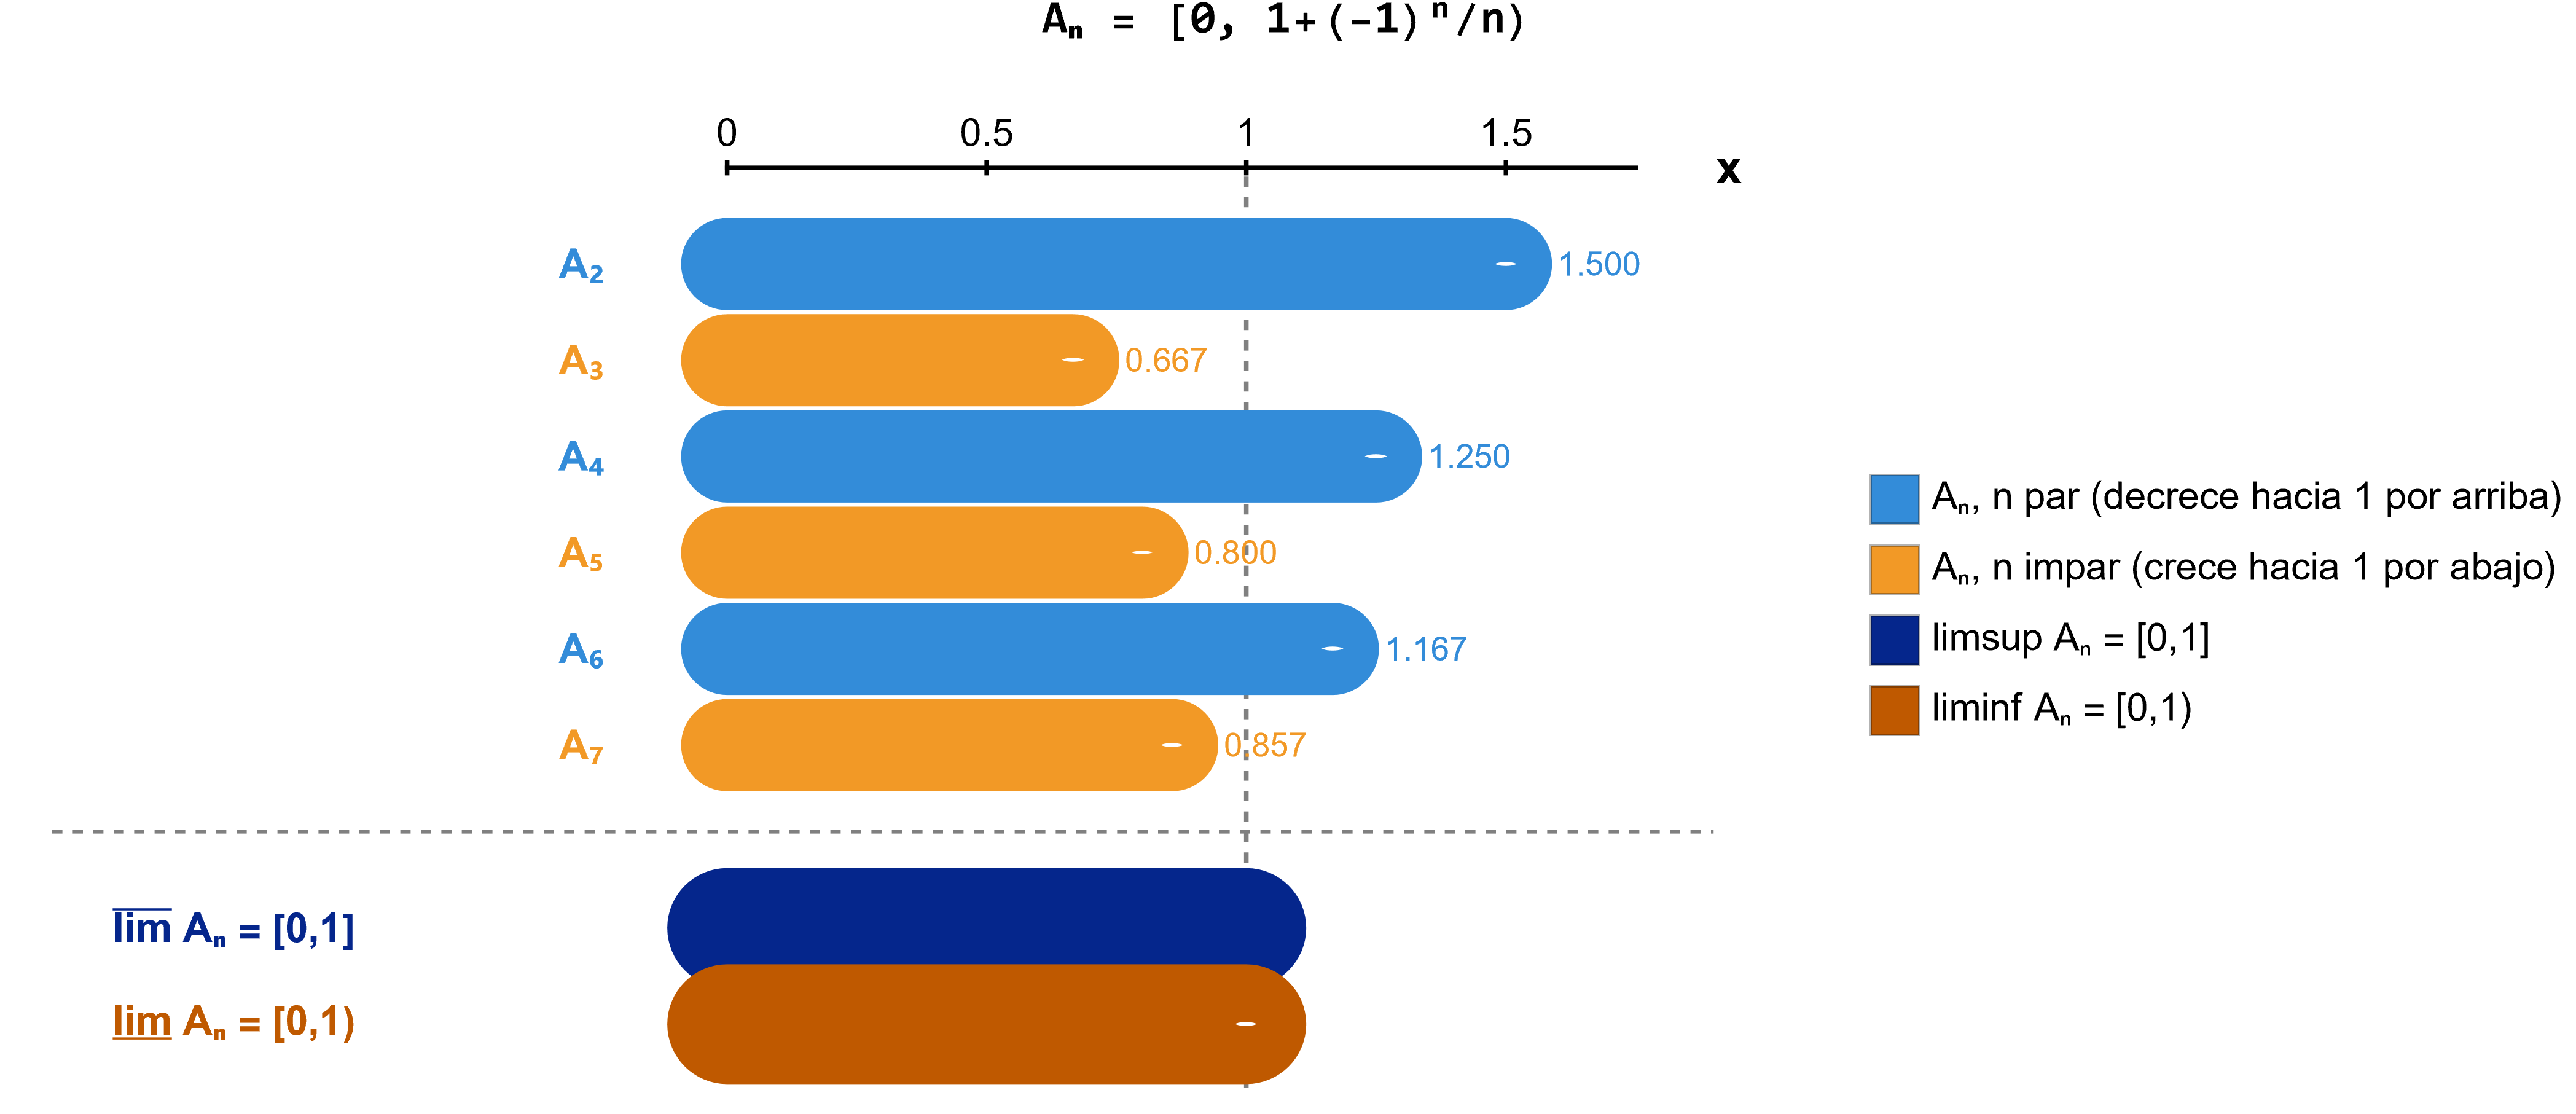
\includegraphics[width=0.85\linewidth]{imagenes/examenes_resueltos/parcial1_P1.png}
\end{center}

Calculamos los límites superior e inferior de la sucesión general $\{A_n\}$:
\begin{enumerate}[label=\arabic*.]
    \item \textbf{Límite superior ($\varlimsup A_n$):}
    \[
        \varlimsup_{n \to \infty} A_n = \bigcap_{n=1}^\infty \left( \bigcup_{j=n}^\infty A_j \right)
    \]
    Para cualquier $n \in \mathbb{N}$, la unión de la cola $\{A_j\}_{j \ge n}$ está dominada por los términos pares superiores, de forma que $\bigcup_{j=n}^\infty A_j = \left[ 0, 1 + \frac{1}{2m_0} \right)$, donde $2m_0$ es el menor par mayor o igual que $n$. Intersecando sobre $n$:
    \[
        \varlimsup_{n \to \infty} A_n = \bigcap_{m=1}^\infty A_{2m} = [0, 1]
    \]

    \item \textbf{Límite inferior ($\varliminf A_n$):}
    \[
        \varliminf_{n \to \infty} A_n = \bigcup_{n=1}^\infty \left( \bigcap_{j=n}^\infty A_j \right)
    \]
    Para cualquier $n \in \mathbb{N}$, la intersección de la cola $\{A_j\}_{j \ge n}$ está acotada por los términos impares inferiores, de forma que $\bigcap_{j=n}^\infty A_j = \left[ 0, 1 - \frac{1}{2m_1 - 1} \right)$, donde $2m_1 - 1$ es el primer impar mayor o igual que $n$. Uniendo sobre $n$:
    \[
        \varliminf_{n \to \infty} A_n = \bigcup_{m=1}^\infty A_{2m-1} = [0, 1)
    \]
\end{enumerate}

Puesto que $\varliminf_{n \to \infty} A_n = [0, 1) \neq [0, 1] = \varlimsup_{n \to \infty} A_n$, la sucesión no es convergente y \textbf{no existe} el límite $\lim_{n \to \infty} A_n$.
\end{problema}
\newpage
% ------------------------------------------------------------------------------
% PROBLEMA 2
% ------------------------------------------------------------------------------
\begin{problema}[Límites de una sucesión de conjuntos disjuntos dos a dos]
Sea $\Omega$ un conjunto y $\{A_n\}_{n \in \mathbb{N}}$ una sucesión de subconjuntos de $\Omega$ formada por conjuntos disjuntos dos a dos ($A_i \cap A_j = \varnothing$ para todo $i \neq j$). Hallar los límites superior e inferior y determinar si existe el límite de la sucesión $\{A_n\}$.

\tcblower

\paragraph{1. Cálculo del límite inferior ($\varliminf A_n$):}
Por definición, el límite inferior es la unión numerable de las intersecciones de las colas:
\[
    \varliminf_{n \to \infty} A_n = \bigcup_{n=1}^\infty \left( \bigcap_{j=n}^\infty A_j \right)
\]
Para cualquier $n \in \mathbb{N}$ fijo, intersecamos los términos a partir del índice $n$:
\[
    \bigcap_{j=n}^\infty A_j \subseteq A_n \cap A_{n+1}
\]
Como los conjuntos son disjuntos dos a dos, $A_n \cap A_{n+1} = \varnothing$, lo que implica que $\bigcap_{j=n}^\infty A_j = \varnothing$ para todo $n \in \mathbb{N}$. Por tanto:
\[
    \varliminf_{n \to \infty} A_n = \bigcup_{n=1}^\infty \varnothing = \varnothing
\]

\paragraph{2. Cálculo del límite superior ($\varlimsup A_n$):}
El límite superior se define como el conjunto formado por los elementos de $\Omega$ que pertenecen a infinitos conjuntos de la sucesión $\{A_n\}$:
\[
    \varlimsup_{n \to \infty} A_n = \{ \omega \in \Omega \mid \omega \in A_n \text{ para infinitos valores de } n \}
\]
Dado que la familia $\{A_n\}_{n \in \mathbb{N}}$ está formada por conjuntos mutuamente disjuntos, ningún elemento $\omega \in \Omega$ puede pertenecer a más de un conjunto $A_k$. En consecuencia, ningún elemento puede pertenecer a infinitos términos de la sucesión. Deducimos que:
\[
    \varlimsup_{n \to \infty} A_n = \varnothing
\]

\begin{center}
    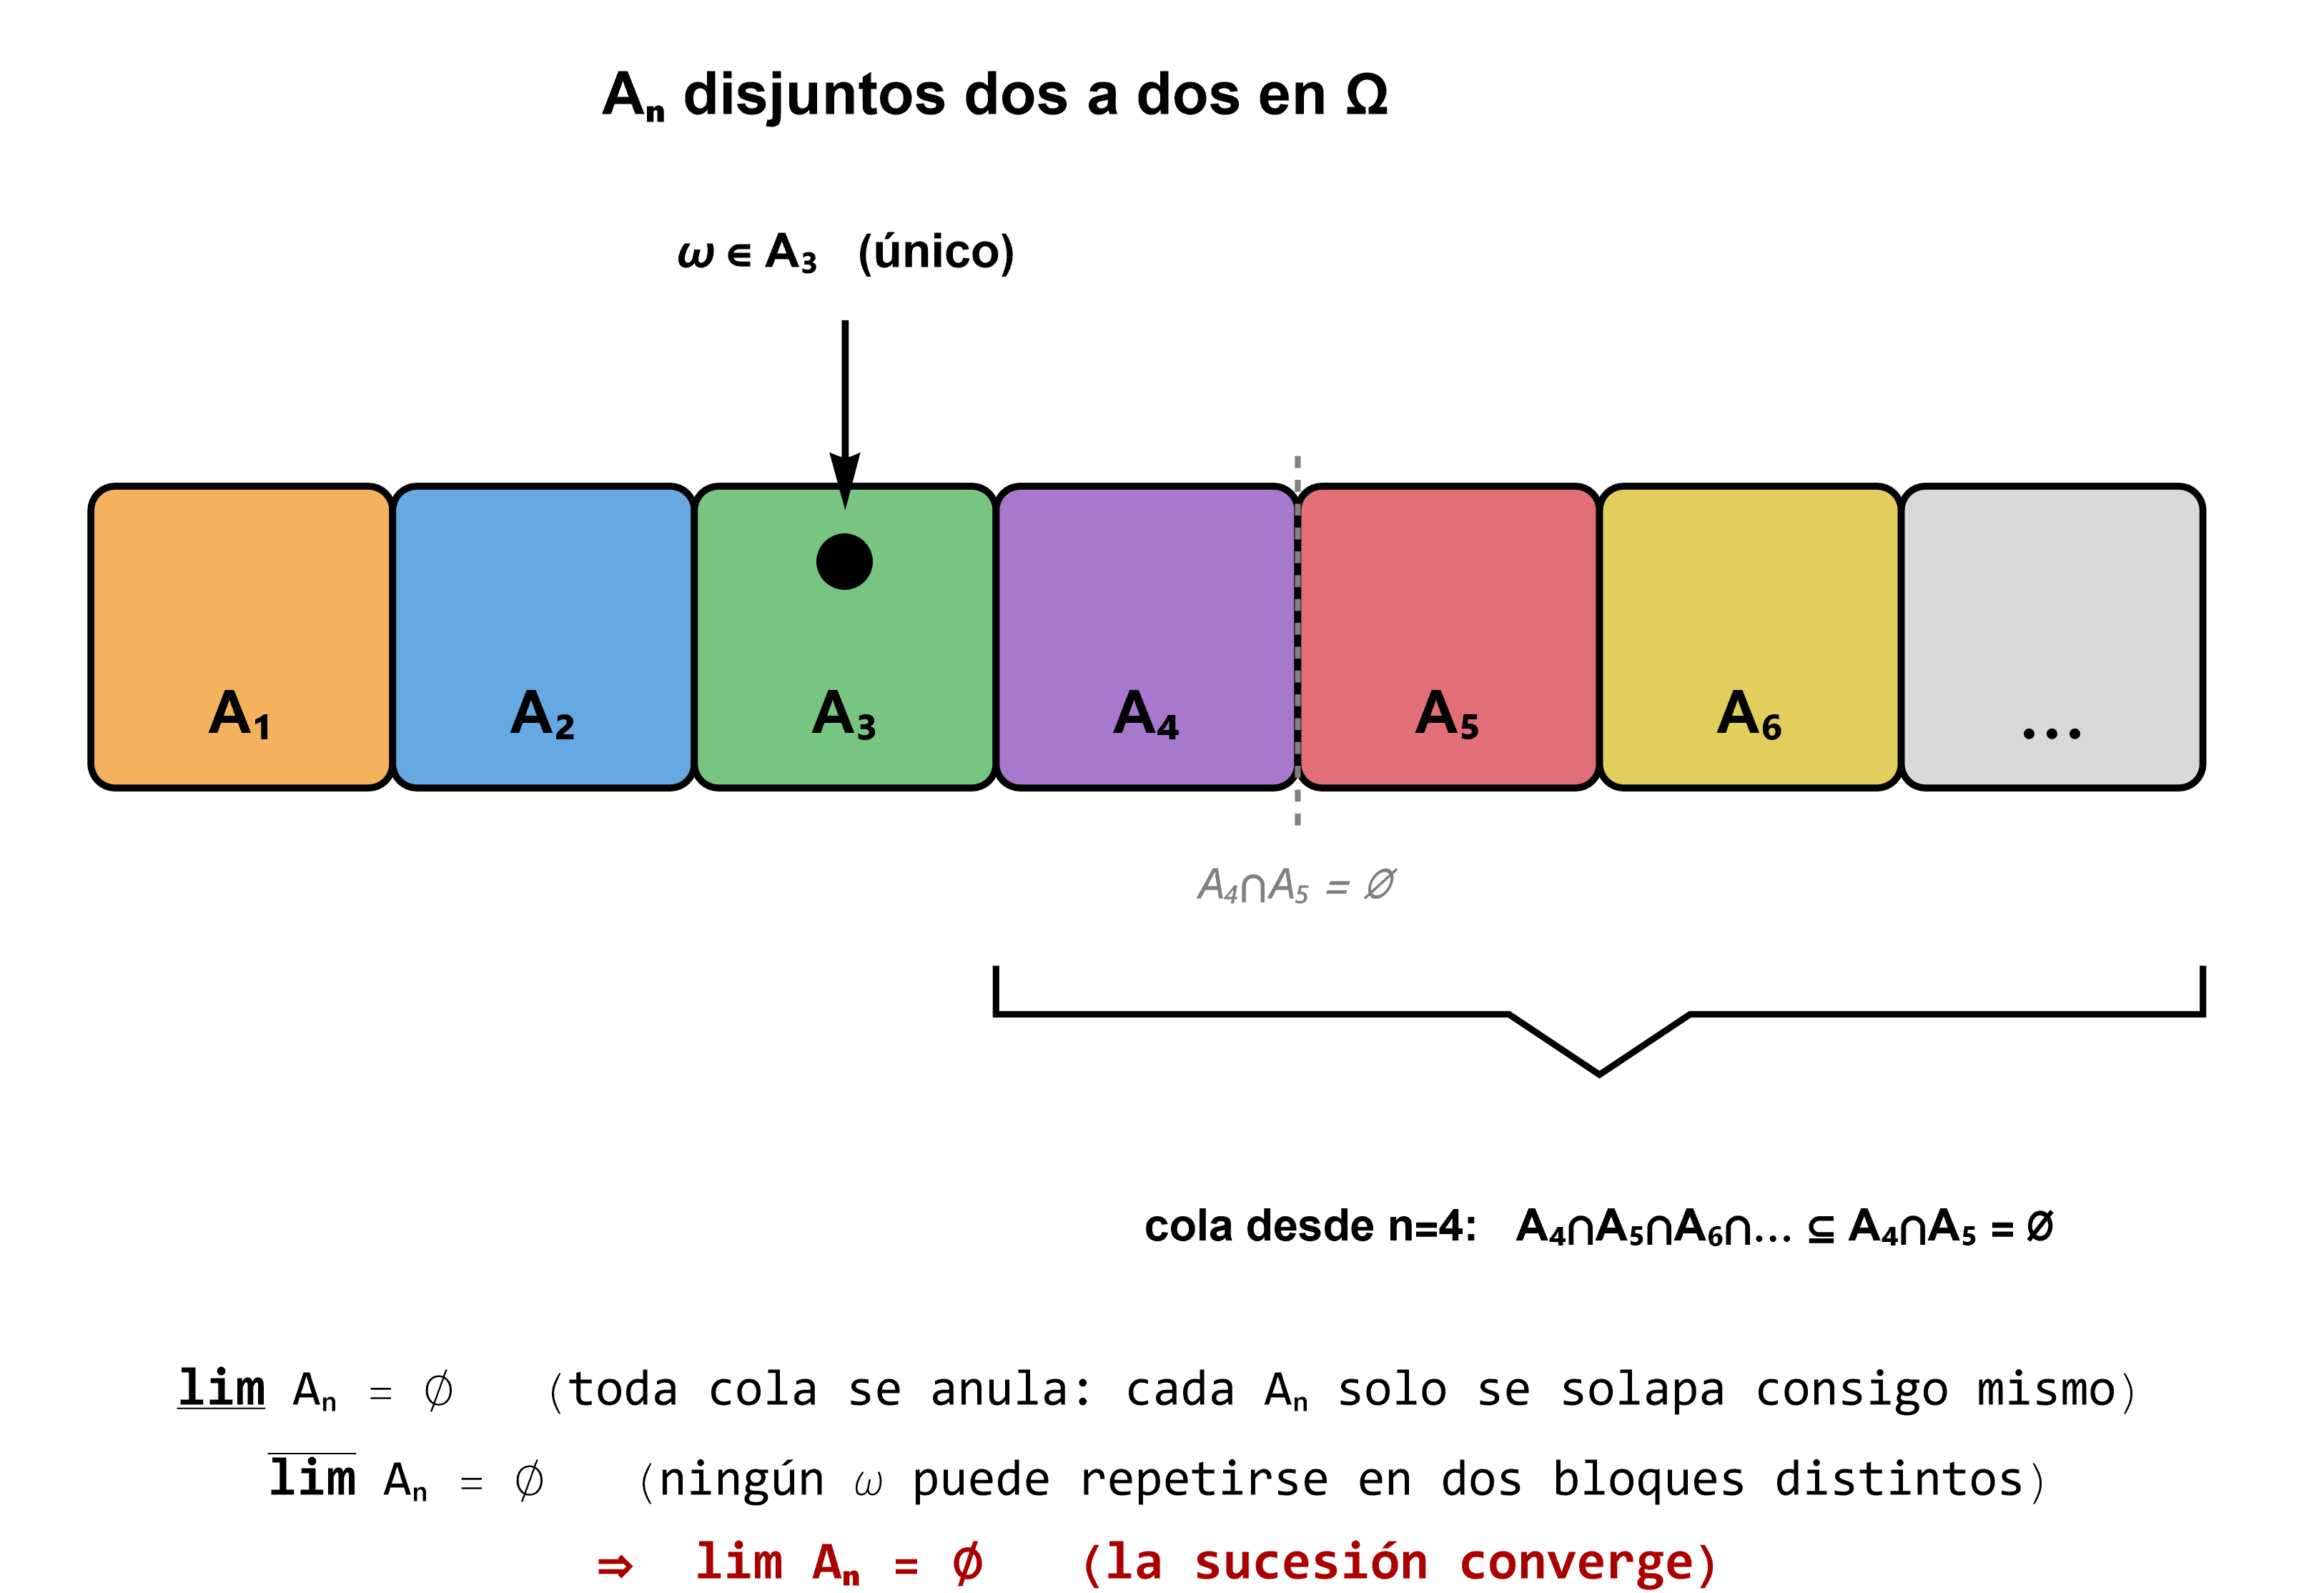
\includegraphics[width=0.65\linewidth]{imagenes/examenes_resueltos/parcial1_P2.png}
\end{center}

\paragraph{3. Existencia del límite de conjuntos:}
Al coincidir los límites inferior y superior:
\[
    \varliminf_{n \to \infty} A_n = \varlimsup_{n \to \infty} A_n = \varnothing
\]
se concluye que la sucesión $\{A_n\}$ es convergente y su límite existe, siendo:
\[
    \lim_{n \to \infty} A_n = \varnothing
\]
\end{problema}

\newpage
% ------------------------------------------------------------------------------
% PROBLEMA 3
% ------------------------------------------------------------------------------
\begin{problema}[Estructura de álgebra caracterizada por la diferencia de conjuntos]
Sea $\Omega$ un conjunto y $\mathcal{A}$ una clase de subconjuntos de $\Omega$ tal que $\Omega \in \mathcal{A}$ y satisface que si $A, B \in \mathcal{A}$, entonces $A \setminus B \in \mathcal{A}$. Demostrar que $\mathcal{A}$ tiene estructura de álgebra sobre $\Omega$.

\tcblower

Recordemos que una familia de subconjuntos $\mathcal{A} \subseteq \mathcal{P}(\Omega)$ es un álgebra sobre $\Omega$ si cumple tres propiedades:
\begin{enumerate}[label=\arabic*.]
    \item $\Omega \in \mathcal{A}$.
    \item Estabilidad por complementación: Si $A \in \mathcal{A} \implies A^c \in \mathcal{A}$.
    \item Estabilidad por uniones finitas: Si $A, B \in \mathcal{A} \implies A \cup B \in \mathcal{A}$.
\end{enumerate}

Comprobamos cada una de las condiciones a partir de las hipótesis dadas:

\paragraph{1. Pertenencia del conjunto total y del conjunto vacío:}
Por hipótesis explícita, $\Omega \in \mathcal{A}$.
Asimismo, aplicando la propiedad de cierre por diferencia a $A = B = \Omega \in \mathcal{A}$:
\[
    \varnothing = \Omega \setminus \Omega \in \mathcal{A}
\]

\paragraph{2. Estabilidad por complementación:}
Sea $A \in \mathcal{A}$ un elemento arbitrario. Expresamos su complementario respecto de $\Omega$ mediante la diferencia de conjuntos:
\[
    A^c = \Omega \setminus A
\]
Como $\Omega \in \mathcal{A}$ y $A \in \mathcal{A}$, la hipótesis de estabilidad por diferencias garantiza que $\Omega \setminus A \in \mathcal{A}$, por lo que $A^c \in \mathcal{A}$.

\paragraph{3. Estabilidad por uniones finitas:}
Sean $A, B \in \mathcal{A}$. Deseamos probar que $A \cup B \in \mathcal{A}$.
\begin{itemize}
    \item Por el paso anterior, al ser $A \in \mathcal{A}$, su complementario $A^c$ pertenece a $\mathcal{A}$.
    \item Como $A^c \in \mathcal{A}$ y $B \in \mathcal{A}$, aplicando la hipótesis de diferencia de conjuntos resulta $A^c \setminus B \in \mathcal{A}$.
    \item Aplicando nuevamente la propiedad del complementario al conjunto $(A^c \setminus B) \in \mathcal{A}$:
    \[
        (A^c \setminus B)^c = \Omega \setminus (A^c \setminus B) \in \mathcal{A}
    \]
\end{itemize}

\begin{center}
    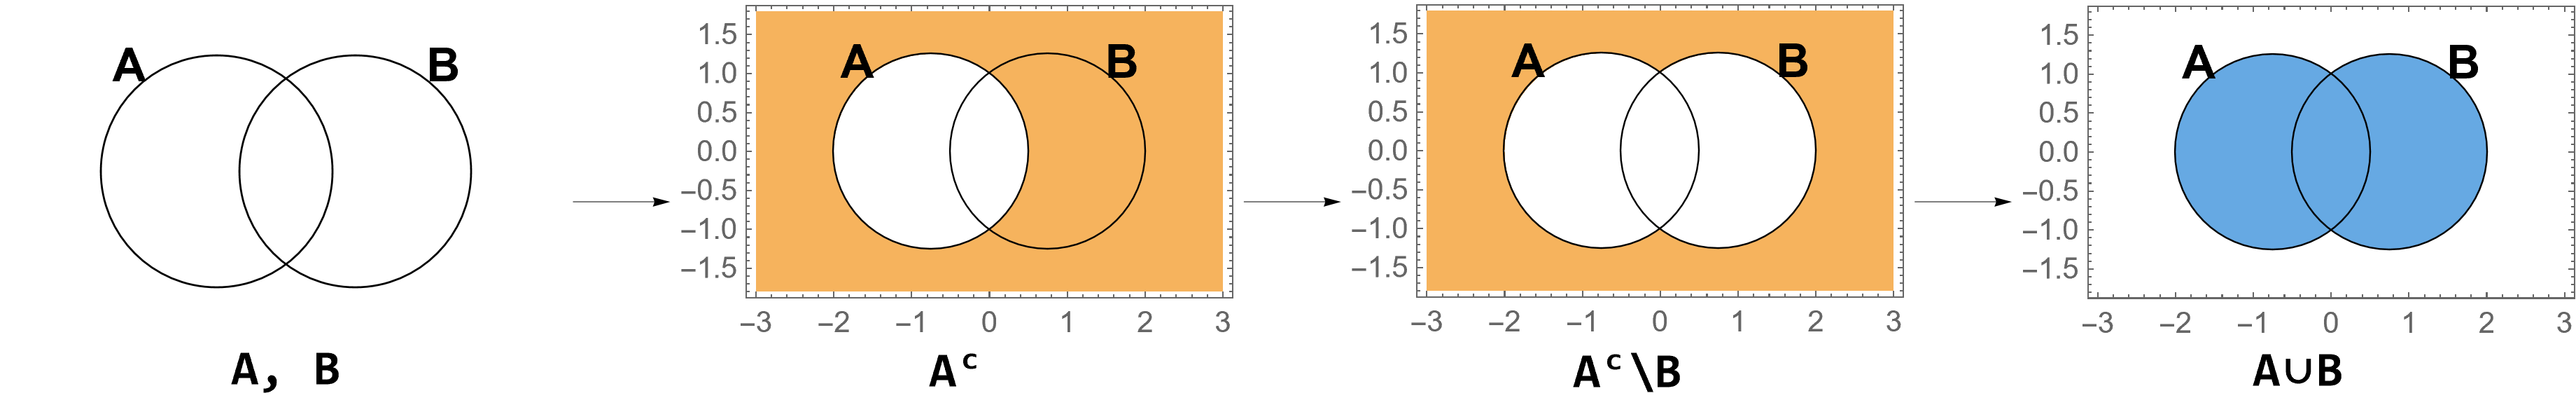
\includegraphics[width=0.95\linewidth]{imagenes/examenes_resueltos/parcial1_P3.png}
\end{center}

Simplificamos la expresión $(A^c \setminus B)^c$ aplicando las leyes de De Morgan:
\[
    (A^c \setminus B)^c = (A^c \cap B^c)^c = (A^c)^c \cup (B^c)^c = A \cup B
\]
Dado que $(A^c \setminus B)^c \in \mathcal{A}$, se deduce que $A \cup B \in \mathcal{A}$.

\paragraph{Conclusión:}
Al verificarse los tres axiomas, queda demostrado que $\mathcal{A}$ es un álgebra sobre $\Omega$.
\end{problema}
\newpage
% ------------------------------------------------------------------------------
% PROBLEMA 4
% ------------------------------------------------------------------------------
\begin{problema}[Comprobación de la medida de probabilidad de Dirac]
Sea $(\Omega, \mathcal{G})$ un espacio medible. Dado un punto fijo $x_0 \in \Omega$, se define la función de conjunto $\delta_{x_0} : \mathcal{G} \to \mathbb{R}$ (masa o medida de Dirac concentrada en $x_0$) como:
\[
    \delta_{x_0}(E) = \begin{cases} 1 & \text{si } x_0 \in E \\ 0 & \text{si } x_0 \notin E \end{cases}, \quad \forall E \in \mathcal{G}
\]
Demostrar que $\delta_{x_0}$ es una medida de probabilidad sobre $(\Omega, \mathcal{G})$.

\tcblower

Verificamos los axiomas de Kolmogorov para demostrar que $\delta_{x_0}$ es una medida de probabilidad sobre $(\Omega, \mathcal{G})$:

\paragraph{1. No negatividad:}
Por definición, para cualquier suceso medible $E \in \mathcal{G}$, la función toma valores en $\{0, 1\}$:
\[
    \delta_{x_0}(E) \ge 0, \quad \forall E \in \mathcal{G}
\]

\paragraph{2. Normalización y conjunto vacío:}
\begin{itemize}
    \item Para el espacio total $\Omega$, como $x_0 \in \Omega$, se satisface:
    \[
        \delta_{x_0}(\Omega) = 1
    \]
    \item Para el conjunto vacío $\varnothing$, dado que $x_0 \notin \varnothing$, resulta:
    \[
        \delta_{x_0}(\varnothing) = 0
    \]
\end{itemize}

\paragraph{3. $\sigma$-aditividad:}
Sea $(E_n)_{n \in \mathbb{N}} \subseteq \mathcal{G}$ una sucesión de conjuntos medibles disjuntos dos a dos ($E_i \cap E_j = \varnothing$ para todo $i \neq j$). Distinguimos dos casos posibles respecto al punto $x_0$:

\begin{enumerate}[label=\alph*)]
    \item \textit{El punto $x_0$ no pertenece a la unión ($x_0 \notin \bigcup_{n=1}^\infty E_n$):}
    Esto implica que $x_0 \notin E_n$ para todo $n \in \mathbb{N}$, por lo que $\delta_{x_0}(E_n) = 0$ para todo $n$. Evaluando ambos miembros:
    \[
        \delta_{x_0}\left( \bigcup_{n=1}^\infty E_n \right) = 0 \quad \text{y} \quad \sum_{n=1}^\infty \delta_{x_0}(E_n) = \sum_{n=1}^\infty 0 = 0
    \]

    \item \textit{El punto $x_0$ pertenece a la unión ($x_0 \in \bigcup_{n=1}^\infty E_n$):}
    Al ser la familia $(E_n)_{n \in \mathbb{N}}$ disjunta dos a dos, existe un \textbf{único} índice $n_0 \in \mathbb{N}$ tal que $x_0 \in E_{n_0}$, y $x_0 \notin E_k$ para todo $k \neq n_0$.
    En consecuencia:
    \[
        \delta_{x_0}(E_{n_0}) = 1 \quad \text{y} \quad \delta_{x_0}(E_k) = 0, \quad \forall k \neq n_0
    \]
    Calculando la suma de las medidas:
    \[
        \sum_{n=1}^\infty \delta_{x_0}(E_n) = \delta_{x_0}(E_{n_0}) + \sum_{k \neq n_0} \delta_{x_0}(E_k) = 1 + 0 = 1
    \]
    Por otra parte, como $x_0 \in \bigcup_{n=1}^\infty E_n$, la medida de la unión es $\delta_{x_0}\left( \bigcup_{n=1}^\infty E_n \right) = 1$.
\end{enumerate}

\begin{center}
    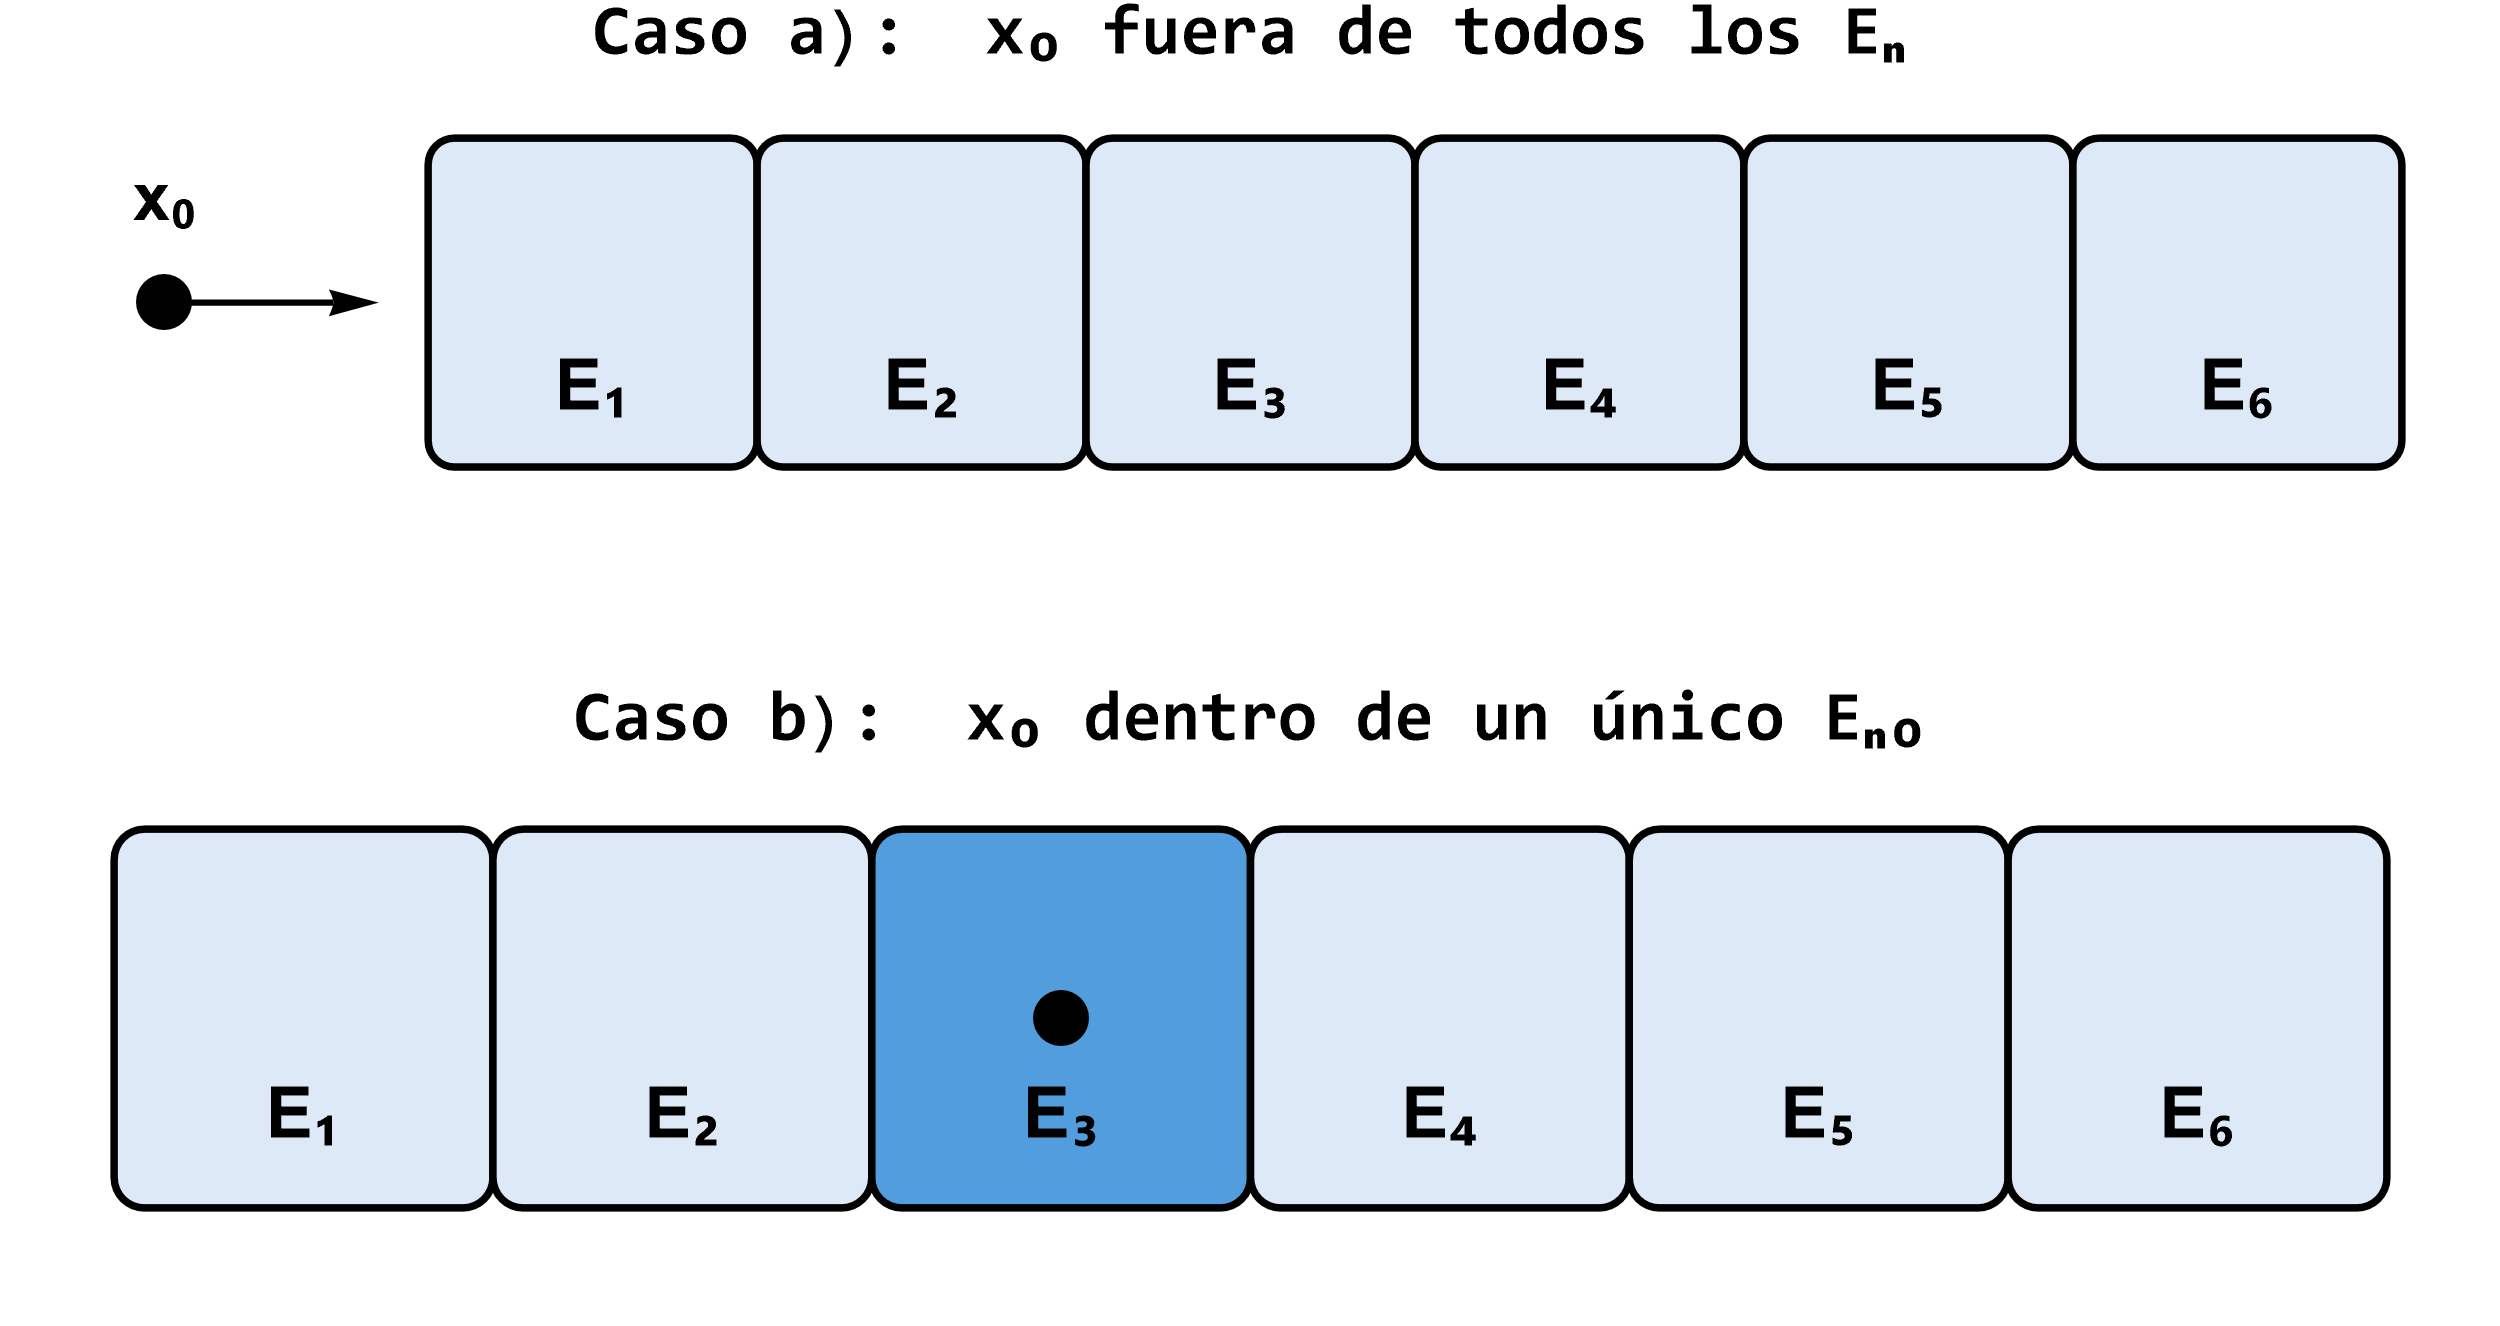
\includegraphics[width=0.55\linewidth]{imagenes/examenes_resueltos/parcial1_P4.png}
\end{center}

En ambos casos se verifica la igualdad $\delta_{x_0}\left( \bigcup_{n=1}^\infty E_n \right) = \sum_{n=1}^\infty \delta_{x_0}(E_n)$.

\paragraph{Conclusión:}
$\delta_{x_0}$ satisface todos los axiomas de Kolmogorov y constituye una medida de probabilidad sobre $(\Omega, \mathcal{G})$.
\end{problema}

\newpage

\section{Otro examen}
\setcounter{problemacontador}{0}
% ------------------------------------------------------------------------------
% PROBLEMA 1
% ------------------------------------------------------------------------------
\begin{problema}[Inclusión y contraejemplo para el límite superior de la intersección de sucesiones de conjuntos]
Sean $\{A_n\}_{n \in \mathbb{N}}$ y $\{B_n\}_{n \in \mathbb{N}}$ dos sucesiones de subconjuntos de un conjunto universal $\Omega$, y consideramos la sucesión formada por sus intersecciones $\{A_n \cap B_n\}_{n \in \mathbb{N}}$.
\begin{enumerate}[label=\alph*)]
    \item Demostrar que se verifica la inclusión:
    \[
        \varlimsup_{n \to \infty} (A_n \cap B_n) \subseteq \varlimsup_{n \to \infty} A_n \cap \varlimsup_{n \to \infty} B_n
    \]
    \item Analizar si se verifica la inclusión recíproca:
    \[
        \varlimsup_{n \to \infty} A_n \cap \varlimsup_{n \to \infty} B_n \subseteq \varlimsup_{n \to \infty} (A_n \cap B_n)
    \]
    y determinar si en general se cumple la igualdad $\varlimsup_{n \to \infty} (A_n \cap B_n) = \varlimsup_{n \to \infty} A_n \cap \varlimsup_{n \to \infty} B_n$.
\end{enumerate}

\tcblower

\paragraph{a) Demostración de la inclusión $\varlimsup_{n \to \infty} (A_n \cap B_n) \subseteq \varlimsup_{n \to \infty} A_n \cap \varlimsup_{n \to \infty} B_n$:}
Recordemos que el límite superior de una sucesión de conjuntos $\{C_n\}_{n \in \mathbb{N}}$ admite la caracterización por elementos:
\[
    \varlimsup_{n \to \infty} C_n = \{ \omega \in \Omega \mid \omega \in C_n \text{ para infinitos valores de } n \in \mathbb{N} \}
\]

Sea $\omega \in \varlimsup_{n \to \infty} (A_n \cap B_n)$ un elemento arbitrario. Por la caracterización elemental del límite superior:
\[
    \omega \in A_n \cap B_n \text{ para infinitos valores de } n \in \mathbb{N}
\]
Por definición de intersección de conjuntos, si $\omega \in A_n \cap B_n$, entonces $\omega \in A_n$ y $\omega \in B_n$ simultáneamente para cada uno de esos infinitos índices $n$. Por tanto:
\begin{itemize}
    \item $\omega \in A_n$ para infinitos índices $n \in \mathbb{N} \implies \omega \in \varlimsup_{n \to \infty} A_n$.
    \item $\omega \in B_n$ para infinitos índices $n \in \mathbb{N} \implies \omega \in \varlimsup_{n \to \infty} B_n$.
\end{itemize}
Al pertenecer $\omega$ a ambos límites superiores, concluimos que:
\[
    \omega \in \varlimsup_{n \to \infty} A_n \cap \varlimsup_{n \to \infty} B_n
\]
Al haberse probado la pertenencia para un elemento arbitrario $\omega$, queda demostrada la inclusión:
\[
    \varlimsup_{n \to \infty} (A_n \cap B_n) \subseteq \varlimsup_{n \to \infty} A_n \cap \varlimsup_{n \to \infty} B_n
\]

\paragraph{b) Análisis de la inclusión recíproca y contraejemplo:}
La inclusión recíproca \textbf{no se verifica en general}. Por consiguiente, la igualdad entre el límite superior de la intersección y la intersección de los límites superiores no se cumple universalmente.

\textit{Contraejemplo:}
Consideremos el espacio universal $\Omega = \{x\}$ con un único elemento y definamos las sucesiones alternadas:
\[
    A_n = \begin{cases} \{x\} & \text{si } n \text{ es impar} \\ \varnothing & \text{si } n \text{ es par} \end{cases}, \qquad B_n = \begin{cases} \varnothing & \text{si } n \text{ es impar} \\ \{x\} & \text{si } n \text{ es par} \end{cases}
\]

Evaluamos los límites superiores de cada sucesión por separado:
\begin{itemize}
    \item En la sucesión $\{A_n\}$, el elemento $x$ pertenece a todos los términos impares $A_1, A_3, A_5, \dots$, que son infinitos. Por tanto:
    \[
        \varlimsup_{n \to \infty} A_n = \{x\}
    \]
    \item En la sucesión $\{B_n\}$, el elemento $x$ pertenece a todos los términos pares $B_2, B_4, B_6, \dots$, que son infinitos. Por tanto:
    \[
        \varlimsup_{n \to \infty} B_n = \{x\}
    \]
\end{itemize}
Intersecando ambos límites superiores obtenemos:
\[
    \varlimsup_{n \to \infty} A_n \cap \varlimsup_{n \to \infty} B_n = \{x\} \cap \{x\} = \{x\}
\]

Por otra parte, calculamos la sucesión intersección $\{A_n \cap B_n\}_{n \in \mathbb{N}}$ término a término. Para cada $n \in \mathbb{N}$, uno de los dos conjuntos es el vacío $\varnothing$, de donde:
\[
    A_n \cap B_n = \varnothing, \quad \forall n \in \mathbb{N}
\]
El límite superior de una sucesión constantemente vacía es el conjunto vacío:
\[
    \varlimsup_{n \to \infty} (A_n \cap B_n) = \varlimsup_{n \to \infty} \varnothing = \varnothing
\]

Puesto que $\{x\} \nsubseteq \varnothing$, se deduce que:
\[
    \varlimsup_{n \to \infty} A_n \cap \varlimsup_{n \to \infty} B_n \nsubseteq \varlimsup_{n \to \infty} (A_n \cap B_n)
\]
demostrándose que la inclusión contraria es falsa en el caso general.

\begin{center}
    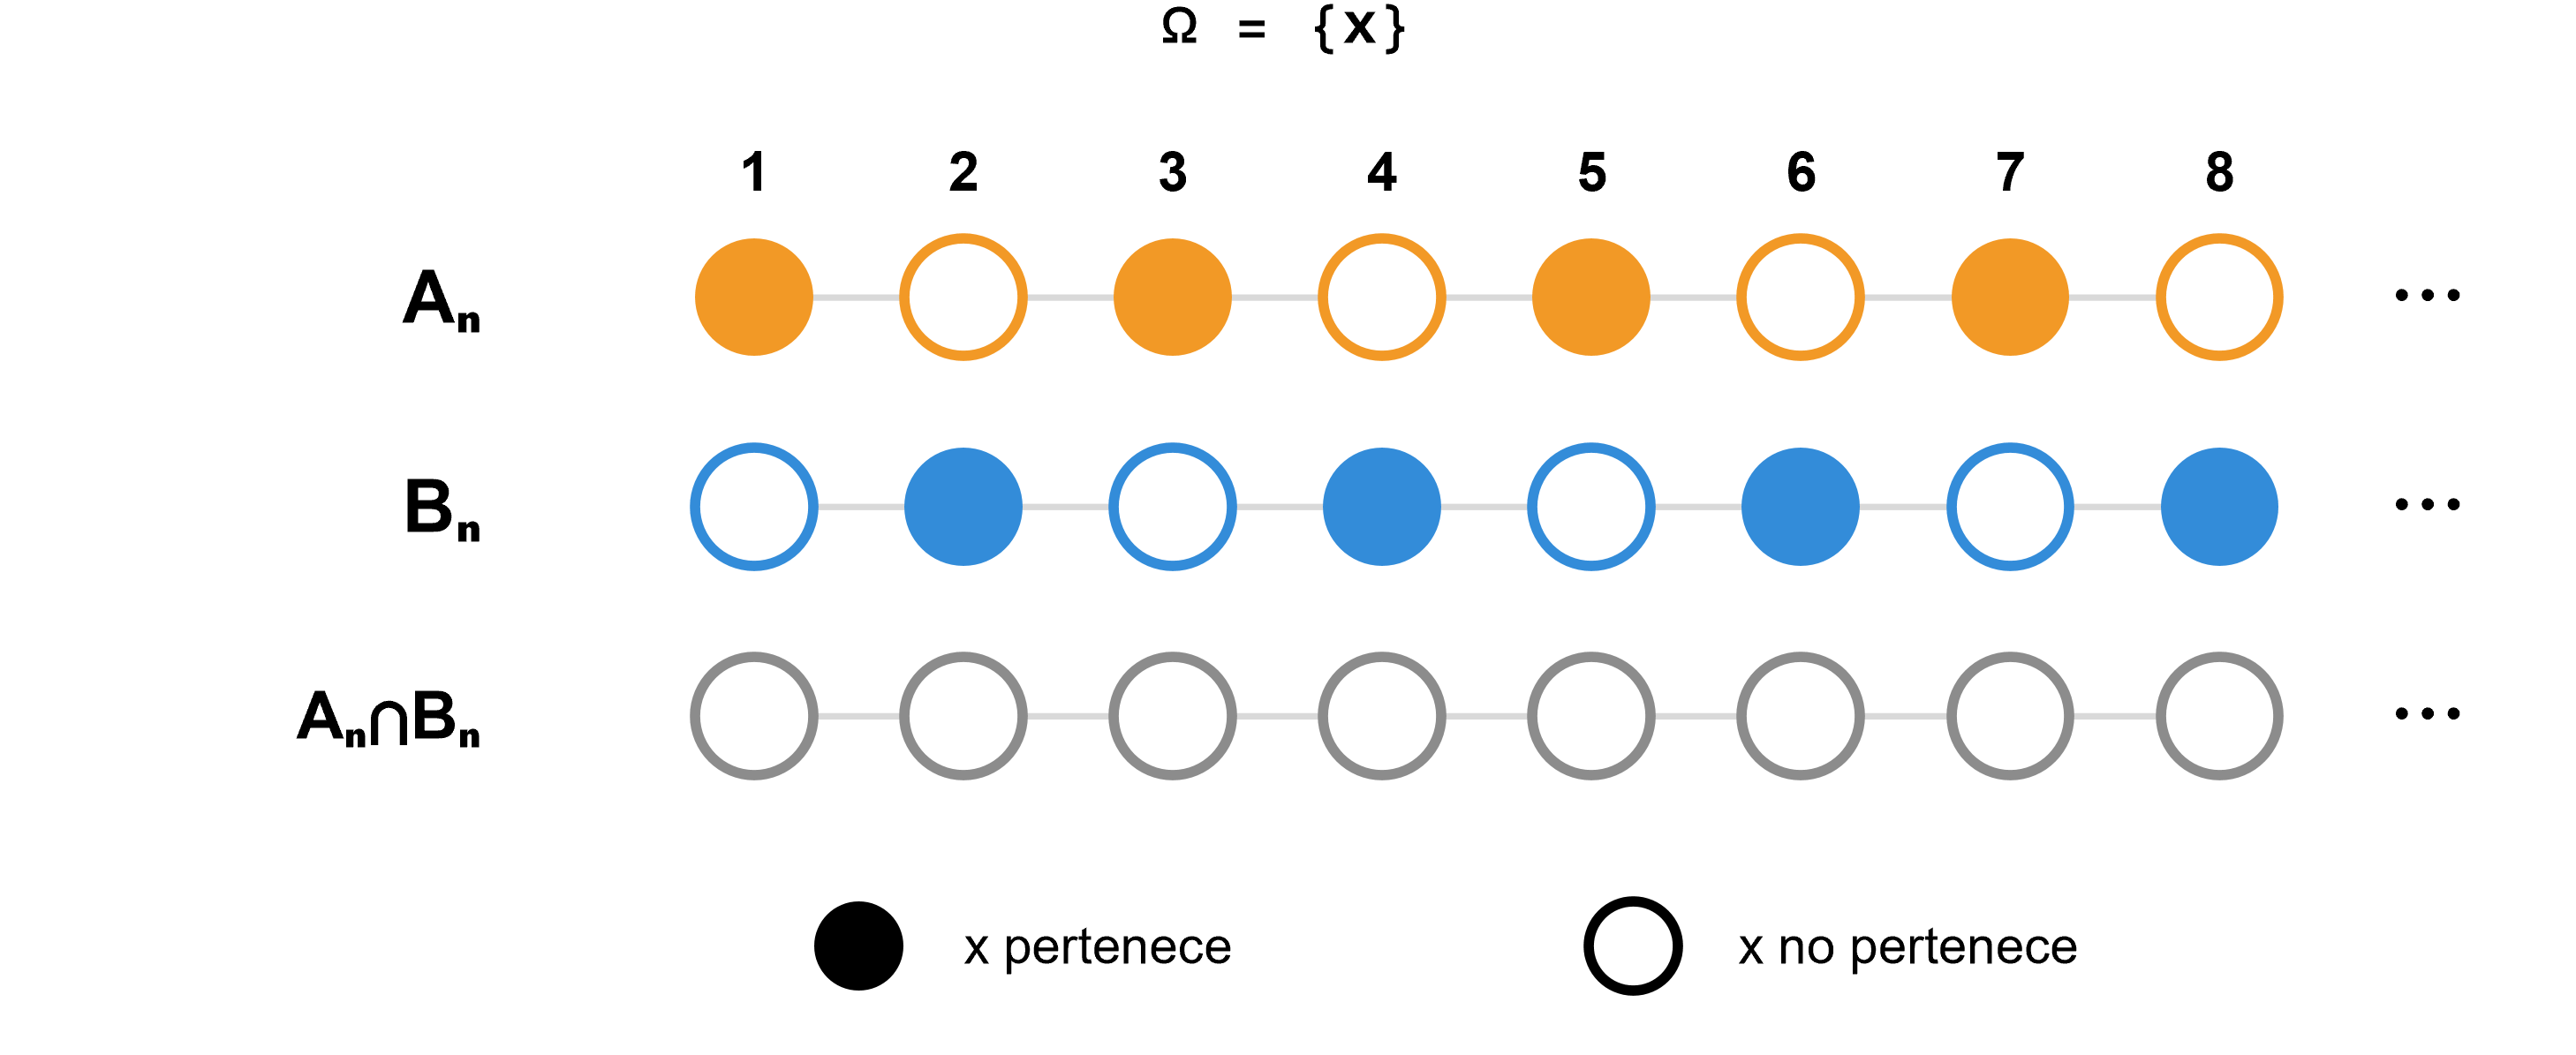
\includegraphics[width=0.55\linewidth]{imagenes/examenes_resueltos/extra1_P1.png}
\end{center}
\end{problema}

% ------------------------------------------------------------------------------
% PROBLEMA 2
% ------------------------------------------------------------------------------
\begin{problema}[Límites superior, inferior y límite de una sucesión de semirrectas no monótonas]
Hallar los límites superior e inferior, y determinar si existe el límite de la sucesión de subconjuntos de $\mathbb{R}$ con término general:
\[
    A_n = \left[ \frac{(-1)^n + n}{n}, \, \infty \right)
\]

\tcblower

Simplificamos la expresión del extremo inferior de cada semirrecta:
\[
    x_n = \frac{(-1)^n + n}{n} = 1 + \frac{(-1)^n}{n} \implies A_n = \left[ 1 + \frac{(-1)^n}{n}, \, \infty \right)
\]

Estudiamos por separado el comportamiento de los términos según la paridad de $n$:
\begin{itemize}
    \item \textbf{Términos impares ($n = 2m - 1$):}
    \[
        A_1 = [0, \infty), \quad A_3 = \left[\frac{2}{3}, \infty\right), \quad A_5 = \left[\frac{4}{5}, \infty\right), \quad \dots, \quad A_{2m-1} = \left[1 - \frac{1}{2m-1}, \infty\right)
    \]
    Los extremos inferiores crecen monótonamente hacia $1$: $\left(1 - \frac{1}{2m-1}\right) \uparrow 1$.

    \item \textbf{Términos pares ($n = 2m$):}
    \[
        A_2 = \left[\frac{3}{2}, \infty\right), \quad A_4 = \left[\frac{5}{4}, \infty\right), \quad A_6 = \left[\frac{7}{6}, \infty\right), \quad \dots, \quad A_{2m} = \left[1 + \frac{1}{2m}, \infty\right)
    \]
    Los extremos inferiores decrecen monótonamente hacia $1$: $\left(1 + \frac{1}{2m}\right) \downarrow 1$.
\end{itemize}

\begin{center}
    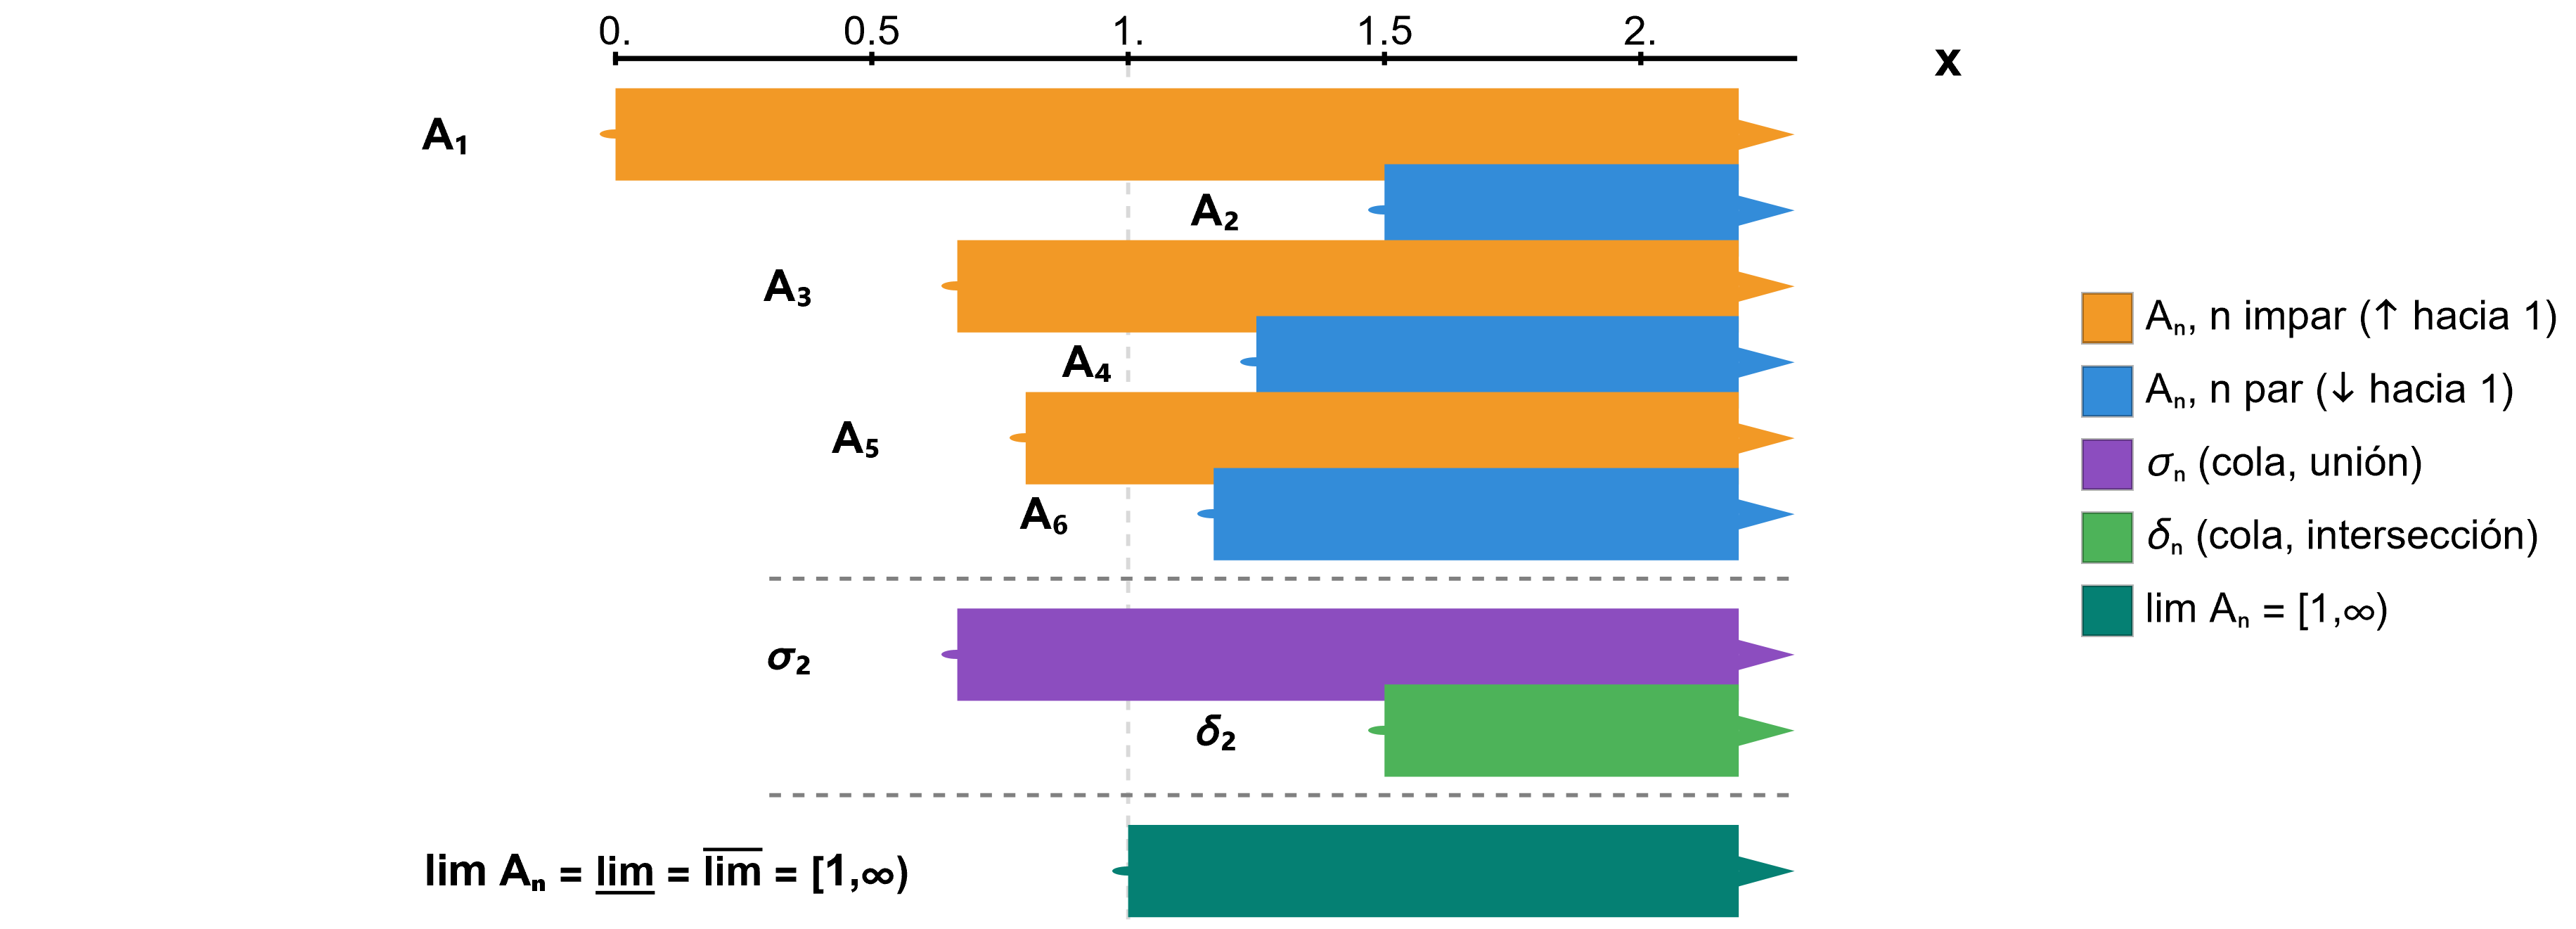
\includegraphics[width=0.55\linewidth]{imagenes/examenes_resueltos/extra1_P2.png}
\end{center}

\paragraph{1. Cálculo de las sucesiones de cola $\sigma_n$ y $\delta_n$:}
\begin{itemize}
    \item \textit{Sucesión de uniones de cola $\sigma_n = \bigcup_{j=n}^\infty A_j$:}
    La unión de una familia de semirrectas $[x_j, \infty)$ viene dada por $\left[ \inf_{j \ge n} x_j, \infty \right)$.
    Para cualquier $n \in \mathbb{N}$, el ínfimo de los extremos a partir del índice $n$ se alcanza siempre en el primer término impar mayor o igual que $n$:
    \begin{align*}
        \sigma_1 &= A_1 \cup A_2 \cup A_3 \cup \dots = [0, \infty) \\
        \sigma_2 &= A_2 \cup A_3 \cup A_4 \cup \dots = \left[\frac{2}{3}, \infty\right) \\
        \sigma_3 &= A_3 \cup A_4 \cup A_5 \cup \dots = \left[\frac{2}{3}, \infty\right) \\
        \sigma_4 &= A_4 \cup A_5 \cup A_6 \cup \dots = \left[\frac{4}{5}, \infty\right)
    \end{align*}
    En general, la sucesión $\{\sigma_n\}$ es una sucesión decreciente de conjuntos ($\sigma_n \downarrow$).

    \item \textit{Sucesión de intersecciones de cola $\delta_n = \bigcap_{j=n}^\infty A_j$:}
    La intersección de una familia de semirrectas $[x_j, \infty)$ viene dada por $\left[ \sup_{j \ge n} x_j, \infty \right)$.
    Para cualquier $n \in \mathbb{N}$, el supremo de los extremos a partir del índice $n$ se alcanza siempre en el primer término par mayor o igual que $n$:
    \begin{align*}
        \delta_1 &= A_1 \cap A_2 \cap A_3 \cap \dots = \left[\frac{3}{2}, \infty\right) \\
        \delta_2 &= A_2 \cap A_3 \cap A_4 \cap \dots = \left[\frac{3}{2}, \infty\right) \\
        \delta_3 &= A_3 \cap A_4 \cap A_5 \cap \dots = \left[\frac{5}{4}, \infty\right) \\
        \delta_4 &= A_4 \cap A_5 \cap A_6 \cap \dots = \left[\frac{5}{4}, \infty\right)
    \end{align*}
    En general, la sucesión $\{\delta_n\}$ es una sucesión creciente de conjuntos ($\delta_n \uparrow$).
\end{itemize}

\paragraph{2. Cálculo de los límites superior e inferior:}
\begin{enumerate}[label=\arabic*.]
    \item \textbf{Límite superior ($\varlimsup_{n \to \infty} A_n$):}
    Se obtiene mediante la intersección numerable de la sucesión decreciente de colas $\{\sigma_n\}$:
    \[
        \varlimsup_{n \to \infty} A_n = \bigcap_{n=1}^\infty \sigma_n = \lim_{m \to \infty} \left[ 1 - \frac{1}{2m-1}, \, \infty \right) = [1, \infty)
    \]

    \item \textbf{Límite inferior ($\varliminf_{n \to \infty} A_n$):}
    Se obtiene mediante la unión numerable de la sucesión creciente de colas $\{\delta_n\}$:
    \[
        \varliminf_{n \to \infty} A_n = \bigcup_{n=1}^\infty \delta_n = \lim_{m \to \infty} \left[ 1 + \frac{1}{2m}, \, \infty \right) = [1, \infty)
    \]
\end{enumerate}

\paragraph{3. Existencia del límite de la sucesión de conjuntos:}
Al coincidir el límite inferior y el límite superior:
\[
    \varliminf_{n \to \infty} A_n = \varlimsup_{n \to \infty} A_n = [1, \infty)
\]
se concluye que la sucesión $\{A_n\}$ es convergente y su límite existe, siendo:
\[
    \lim_{n \to \infty} A_n = [1, \infty)
\]
\end{problema}
\newpage

\section{Examen Propuesto 1}
\setcounter{problemacontador}{0}
% ------------------------------------------------------------------------------
% PROBLEMA 1
% ------------------------------------------------------------------------------
\begin{problema}[Límites superior e inferior de una sucesión oscilante de intervalos]
Sea $(\mathbb{R}, \mathcal{B})$ el espacio medible boreliano. Se considera la sucesión de subconjuntos de $\mathbb{R}$ dada por:
\[
    A_n = \left[ 1 - \frac{(-1)^n}{n}, \, 2 + \frac{1}{n} \right), \quad \forall n \ge 1
\]
\begin{enumerate}[label=\alph*)]
    \item Determinar de forma razonada las expresiones de las sucesiones de cola $\sigma_n = \bigcup_{j=n}^\infty A_j$ y $\delta_n = \bigcap_{j=n}^\infty A_j$.
    \item Calcular los límites superior e inferior de la sucesión, $\varlimsup_{n \to \infty} A_n$ y $\varliminf_{n \to \infty} A_n$.
    \item Discutir si existe el límite de la sucesión de conjuntos $\lim_{n \to \infty} A_n$.
\end{enumerate}

\tcblower

\paragraph{a) Estudio de las sucesiones de cola $\sigma_n$ y $\delta_n$:}
Analizamos por separado los términos pares e impares del término general $A_n$:
\begin{itemize}
    \item Si $n = 2m$ (par): $A_{2m} = \left[ 1 - \frac{1}{2m}, \, 2 + \frac{1}{2m} \right)$.
    \item Si $n = 2m-1$ (impar): $A_{2m-1} = \left[ 1 + \frac{1}{2m-1}, \, 2 + \frac{1}{2m-1} \right)$.
\end{itemize}

Para la sucesión de uniones de las colas $\sigma_n = \bigcup_{j=n}^\infty A_j$:
\begin{itemize}
    \item El extremo inferior de la unión viene determinado por el mínimo de los extremos inferiores a partir del índice $n$, el cual se alcanza en los términos pares: $\inf_{j \ge n} \left( 1 - \frac{(-1)^j}{j} \right) = 1 - \frac{1}{2 m_0}$, siendo $2 m_0$ el menor entero par mayor o igual que $n$.
    \item El extremo superior de la unión es el supremo de los extremos superiores: $\sup_{j \ge n} \left( 2 + \frac{1}{j} \right) = 2 + \frac{1}{n}$.
\end{itemize}
Por tanto, $\sigma_n = \left[ 1 - \frac{1}{2 \lceil n/2 \rceil}, \, 2 + \frac{1}{n} \right)$.

Para la sucesión de intersecciones de las colas $\delta_n = \bigcap_{j=n}^\infty A_j$:
\begin{itemize}
    \item El extremo inferior de la intersección viene determinado por el supremo de los extremos inferiores a partir de $n$, alcanzado en los términos impares: $\sup_{j \ge n} \left( 1 - \frac{(-1)^j}{j} \right) = 1 + \frac{1}{2 m_1 - 1}$, siendo $2 m_1 - 1$ el menor entero impar mayor o igual que $n$.
    \item El extremo superior de la intersección es el ínfimo de los extremos superiores: $\inf_{j \ge n} \left( 2 + \frac{1}{j} \right) = 2$.
\end{itemize}
Por tanto, $\delta_n = \left[ 1 + \frac{1}{2 \lceil n/2 \rceil - 1}, \, 2 \right]$.

\begin{center}
    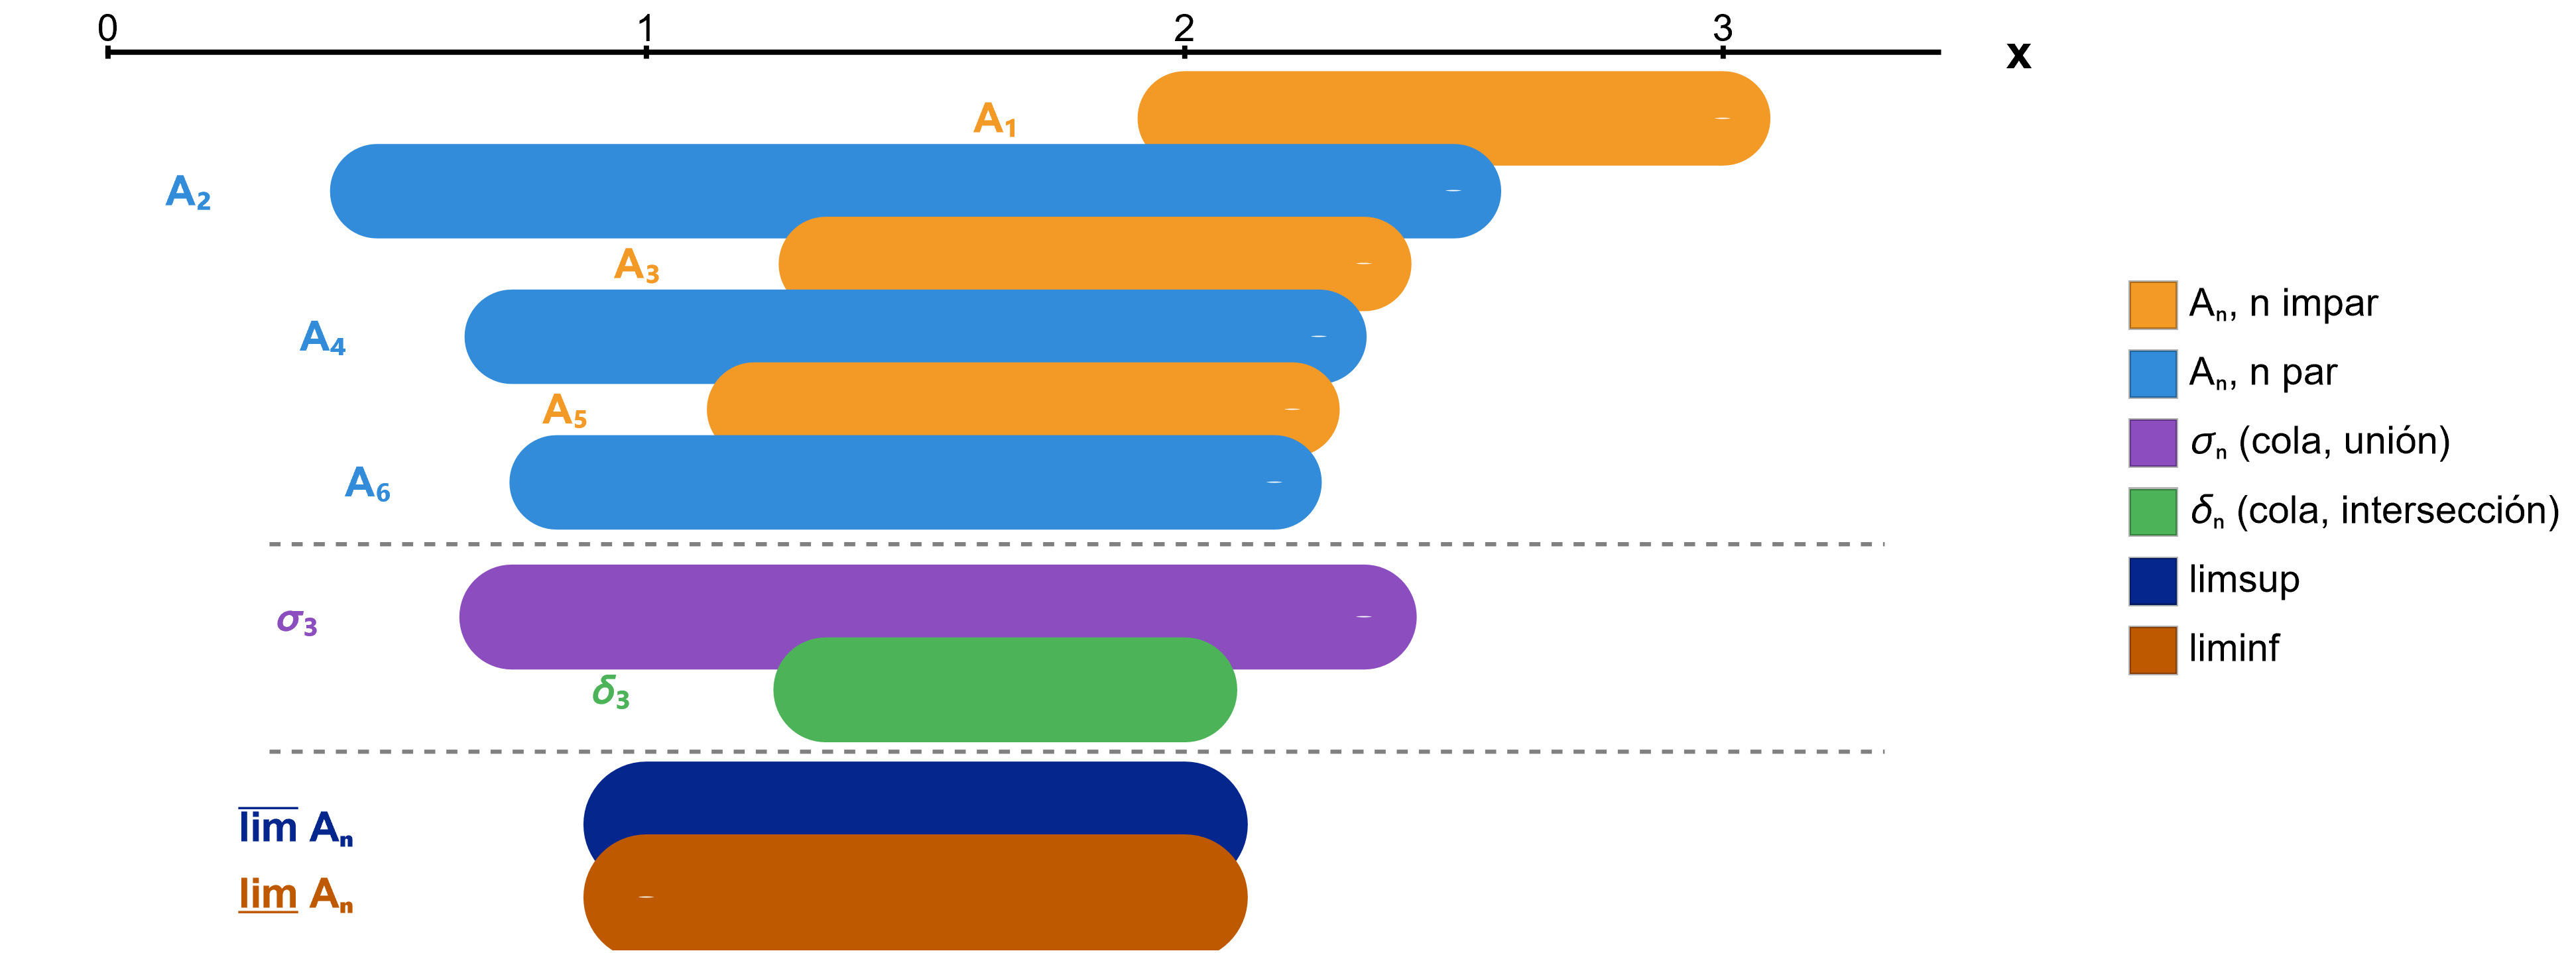
\includegraphics[width=0.85\linewidth]{imagenes/examenes_resueltos/propuesto1_P1.png}
\end{center}

\paragraph{b) Cálculo de los límites superior e inferior:}
\begin{enumerate}[label=\arabic*.]
    \item \textbf{Límite superior ($\varlimsup_{n \to \infty} A_n$):}
    Se obtiene mediante la intersección numerable de la sucesión decreciente de conjuntos $\sigma_n$:
    \[
        \varlimsup_{n \to \infty} A_n = \bigcap_{n=1}^\infty \sigma_n = \bigcap_{n=1}^\infty \left[ 1 - \frac{1}{2 \lceil n/2 \rceil}, \, 2 + \frac{1}{n} \right) = [1, 2]
    \]
    Puesto que para todo $x \in [1,2]$, se cumple $1 - \frac{1}{2 \lceil n/2 \rceil} \le 1 \le x \le 2 < 2 + \frac{1}{n}$ para todo $n \ge 1$.

    \item \textbf{Límite inferior ($\varliminf_{n \to \infty} A_n$):}
    Se obtiene mediante la unión numerable de la sucesión creciente de conjuntos $\delta_n$:
    \[
        \varliminf_{n \to \infty} A_n = \bigcup_{n=1}^\infty \delta_n = \bigcup_{n=1}^\infty \left[ 1 + \frac{1}{2 \lceil n/2 \rceil - 1}, \, 2 \right] = (1, 2]
    \]
    El punto $x = 1$ no pertenece a ningún $\delta_n$ pues $1 < 1 + \frac{1}{2m-1}$ para todo $m \ge 1$.
\end{enumerate}

\paragraph{c) Discusión sobre la existencia del límite:}
Puesto que los límites inferior y superior no coinciden:
\[
    \varliminf_{n \to \infty} A_n = (1, 2] \neq [1, 2] = \varlimsup_{n \to \infty} A_n
\]
se concluye que la sucesión de conjuntos $\{A_n\}$ no es convergente y \textbf{no existe} el límite $\lim_{n \to \infty} A_n$.
\end{problema}

\newpage %===

% ------------------------------------------------------------------------------
% PROBLEMA 2
% ------------------------------------------------------------------------------
\begin{problema}[Teorema de descomposición de Lebesgue y derivada de Radon-Nikodym]
En el espacio medible $(\mathbb{R}, \mathcal{B})$, se consideran las medidas $\mu$ y $\nu$ definidas para cada $A \in \mathcal{B}$ por:
\[
    \mu(A) = \lambda(A \cap [0, 2]) \quad \text{y} \quad \nu(A) = \lambda(A \cap [1, 3]) + \delta_1(A)
\]
donde $\lambda$ representa la medida de Lebesgue y $\delta_1$ la medida de Dirac concentrada en $x = 1$.
\begin{enumerate}[label=\alph*)]
    \item Estudiar la relación de continuidad absoluta o singularidad entre $\mu$ y $\nu$.
    \item Hallar la descomposición de Lebesgue de $\nu$ respecto de $\mu$, identificando explícitamente sus componentes singular ($\nu_1 \perp \mu$) y absolutamente continua ($\nu_2 \ll \mu$).
    \item Calcular la derivada de Radon-Nikodym $\frac{d\nu_2}{d\mu}$.
\end{enumerate}

\tcblower

\paragraph{a) Análisis previo de los soportes y relaciones entre las medidas:}
Observamos que los conjuntos de medida nula según $\mu$ cumplen:
\[
    \mu(A) = 0 \iff \lambda(A \cap [0, 2]) = 0
\]
\begin{itemize}
    \item $\mu$ no es absolutamente continua respecto de $\nu$ ($\mu \not\ll \nu$), pues para $A = (0, 1/2)$, $\nu(A) = 0$ mientras que $\mu(A) = 1/2 > 0$.
    \item $\nu$ no es absolutamente continua respecto de $\mu$ ($\nu \not\ll \mu$), pues para $A = \{1\}$, $\mu(\{1\}) = 0$ mientras que $\nu(\{1\}) = 1 > 0$. Además, para $A = (2, 3]$, $\mu((2,3]) = 0$ mientras que $\nu((2,3]) = 1 > 0$.
\end{itemize}

\paragraph{b) Construcción de la descomposición de Lebesgue ($\nu = \nu_1 + \nu_2$):}
Buscamos dos medidas $\nu_1, \nu_2$ tales que $\nu = \nu_1 + \nu_2$ con $\nu_1 \perp \mu$ y $\nu_2 \ll \mu$.

Consideremos el suceso $S = \{1\} \cup (2, 3] \in \mathcal{B}$. Evaluamos la medida $\mu$ sobre $S$:
\[
    \mu(S) = \mu(\{1\}) + \mu((2, 3]) = \lambda(\{1\} \cap [0,2]) + \lambda((2,3] \cap [0,2]) = 0 + 0 = 0
\]
Definimos la componente singular $\nu_1$ restringiendo $\nu$ al conjunto $S$:
\[
    \nu_1(A) = \nu(A \cap S) = \delta_1(A) + \lambda(A \cap (2, 3]), \quad \forall A \in \mathcal{B}
\]
Verificamos las condiciones de singularidad mutua ($\nu_1 \perp \mu$):
\begin{itemize}
    \item $\mu(S) = 0$.
    \item $\nu_1(S^c) = \nu_1(\mathbb{R} \setminus S) = \delta_1(S^c) + \lambda(S^c \cap (2,3]) = 0 + 0 = 0$.
\end{itemize}
Al existir $S \in \mathcal{B}$ tal que $\mu(S) = 0$ y $\nu_1(S^c) = 0$, se concluye que $\nu_1 \perp \mu$.

\begin{center}
    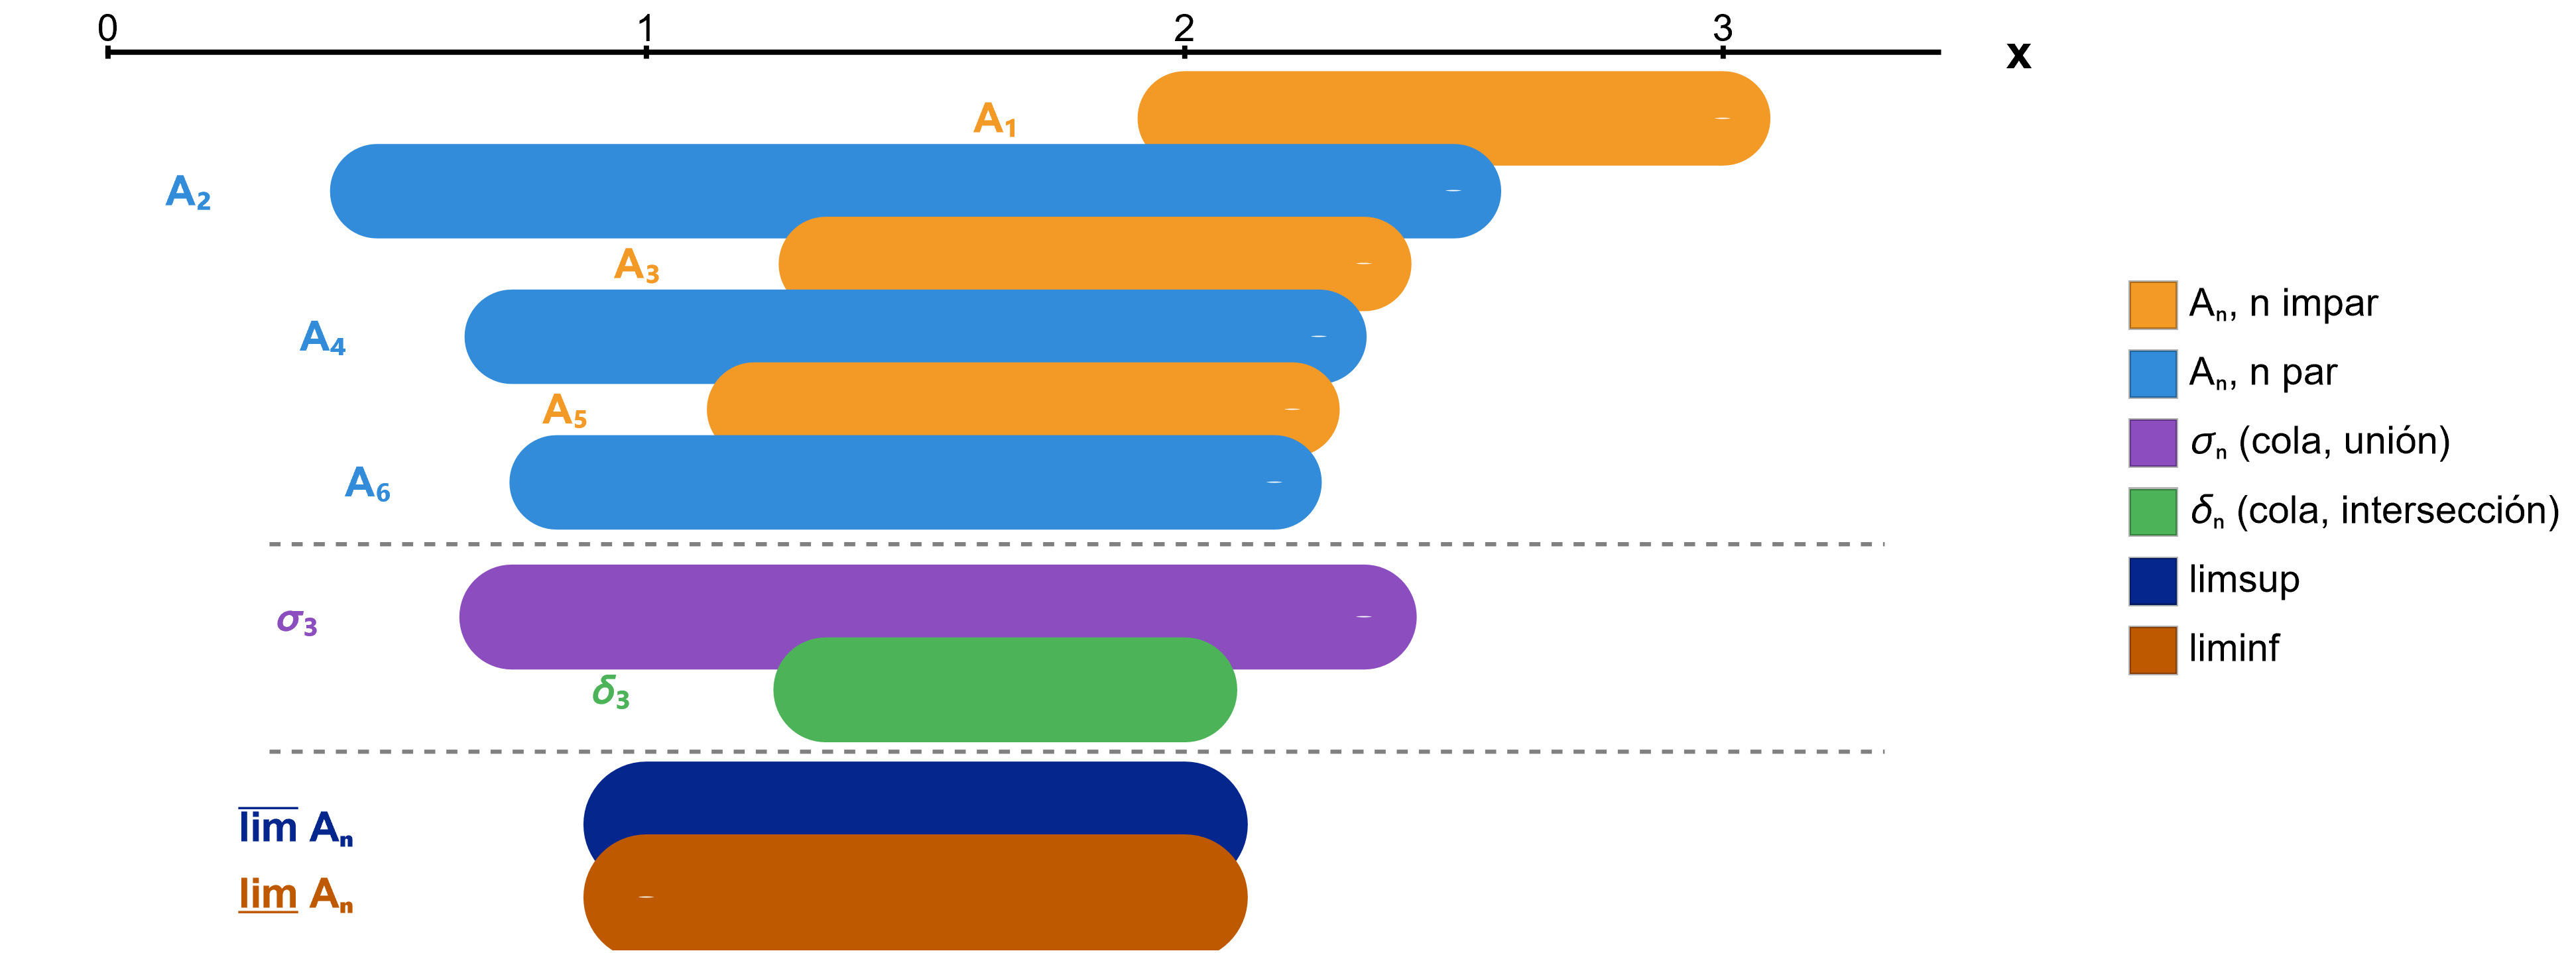
\includegraphics[width=0.85\linewidth]{imagenes/examenes_resueltos/propuesto1_P1.png}
\end{center}

Definimos la componente residual $\nu_2$ restringiendo $\nu$ al complementario $S^c$:
\[
    \nu_2(A) = \nu(A \cap S^c) = \lambda(A \cap ([1, 3] \setminus S)) = \lambda(A \cap [1, 2]), \quad \forall A \in \mathcal{B}
\]
Comprobamos que $\nu_2 \ll \mu$:
Sea $A \in \mathcal{B}$ tal que $\mu(A) = 0 \implies \lambda(A \cap [0, 2]) = 0$. Puesto que $A \cap [1, 2] \subseteq A \cap [0, 2]$, por monotonía de la medida de Lebesgue:
\[
    \nu_2(A) = \lambda(A \cap [1, 2]) \le \lambda(A \cap [0, 2]) = 0 \implies \nu_2(A) = 0
\]
Por lo tanto, $\nu_2 \ll \mu$. La descomposición única de Lebesgue es $\nu = \nu_1 + \nu_2$.

\paragraph{c) Cálculo de la derivada de Radon-Nikodym $\frac{d\nu_2}{d\mu}$:}
Buscamos una función medible $f \ge 0$ tal que $\nu_2(A) = \int_A f(x) \, d\mu(x)$ para todo $A \in \mathcal{B}$.
Observamos que para cualquier $A \subseteq [0,2]$:
\[
    \nu_2(A) = \lambda(A \cap [1, 2]) = \int_A \mathbf{1}_{[1,2]}(x) \, d\lambda(x) = \int_A \mathbf{1}_{[1,2]}(x) \, d\mu(x)
\]
Por la unicidad casi seguro de la derivada de Radon-Nikodym:
\[
    \frac{d\nu_2}{d\mu}(x) = \mathbf{1}_{[1,2]}(x) \quad \text{c.s. } \mu
\]
\end{problema}

\newpage %===

% ------------------------------------------------------------------------------
% PROBLEMA 3
% ------------------------------------------------------------------------------
\begin{problema}[$\sigma$-álgebra imagen inversa y medida de probabilidad inducida]
Sean $(\Omega_1, \mathcal{G}_1)$ y $(\Omega_2, \mathcal{G}_2)$ dos espacios medibles y sea $X : \Omega_1 \to \Omega_2$ una aplicación.
\begin{enumerate}[label=\alph*)]
    \item Demostrar que la colección $X^{-1}(\mathcal{G}_2) = \{ X^{-1}(B) \subseteq \Omega_1 \mid B \in \mathcal{G}_2 \}$ es una $\sigma$-álgebra sobre $\Omega_1$.
    \item Si $\mu$ es una medida sobre $(\Omega_1, \mathcal{G}_1)$, demostrar que la función de conjunto $P_X : \mathcal{G}_2 \to \overline{\mathbb{R}}$ definida por $P_X(B) = \mu(X^{-1}(B))$ es una medida sobre $(\Omega_2, \mathcal{G}_2)$.
    \item Demostrar que si $\mu$ es una medida de probabilidad sobre $\Omega_1$, entonces $P_X$ es una medida de probabilidad sobre $\Omega_2$.
\end{enumerate}

\tcblower

\paragraph{a) Demostración de que $X^{-1}(\mathcal{G}_2)$ es una $\sigma$-álgebra sobre $\Omega_1$:}
Comprobamos las tres condiciones constitutivas de una $\sigma$-álgebra:
\begin{enumerate}[label=\arabic*.]
    \item \textbf{Pertenencia del espacio total:} Como $\mathcal{G}_2$ es $\sigma$-álgebra sobre $\Omega_2$, se cumple $\Omega_2 \in \mathcal{G}_2$. Su antiimagen satisface $X^{-1}(\Omega_2) = \Omega_1$, por lo que $\Omega_1 \in X^{-1}(\mathcal{G}_2)$.
    \item \textbf{Estabilidad por complementación:} Sea $A \in X^{-1}(\mathcal{G}_2)$. Por definición, existe un suceso $B \in \mathcal{G}_2$ tal que $A = X^{-1}(B)$. Tomando el complementario respecto a $\Omega_1$:
    \[
        A^c = (X^{-1}(B))^c = X^{-1}(B^c)
    \]
    Como $\mathcal{G}_2$ es $\sigma$-álgebra, $B^c \in \mathcal{G}_2$, de donde se deduce que $A^c \in X^{-1}(\mathcal{G}_2)$.
    \item \textbf{Estabilidad por uniones numerables:} Sea $(A_n)_{n \in \mathbb{N}} \subseteq X^{-1}(\mathcal{G}_2)$ una sucesión de conjuntos. Para cada $n \in \mathbb{N}$, existe $B_n \in \mathcal{G}_2$ tal que $A_n = X^{-1}(B_n)$. Por las propiedades de la imagen inversa:
    \[
        \bigcup_{n=1}^\infty A_n = \bigcup_{n=1}^\infty X^{-1}(B_n) = X^{-1}\left( \bigcup_{n=1}^\infty B_n \right)
    \]
    Dado que $\mathcal{G}_2$ es $\sigma$-álgebra, la unión numerable $\bigcup_{n=1}^\infty B_n \in \mathcal{G}_2$, por lo que $\bigcup_{n=1}^\infty A_n \in X^{-1}(\mathcal{G}_2)$.
\end{enumerate}

\begin{center}
    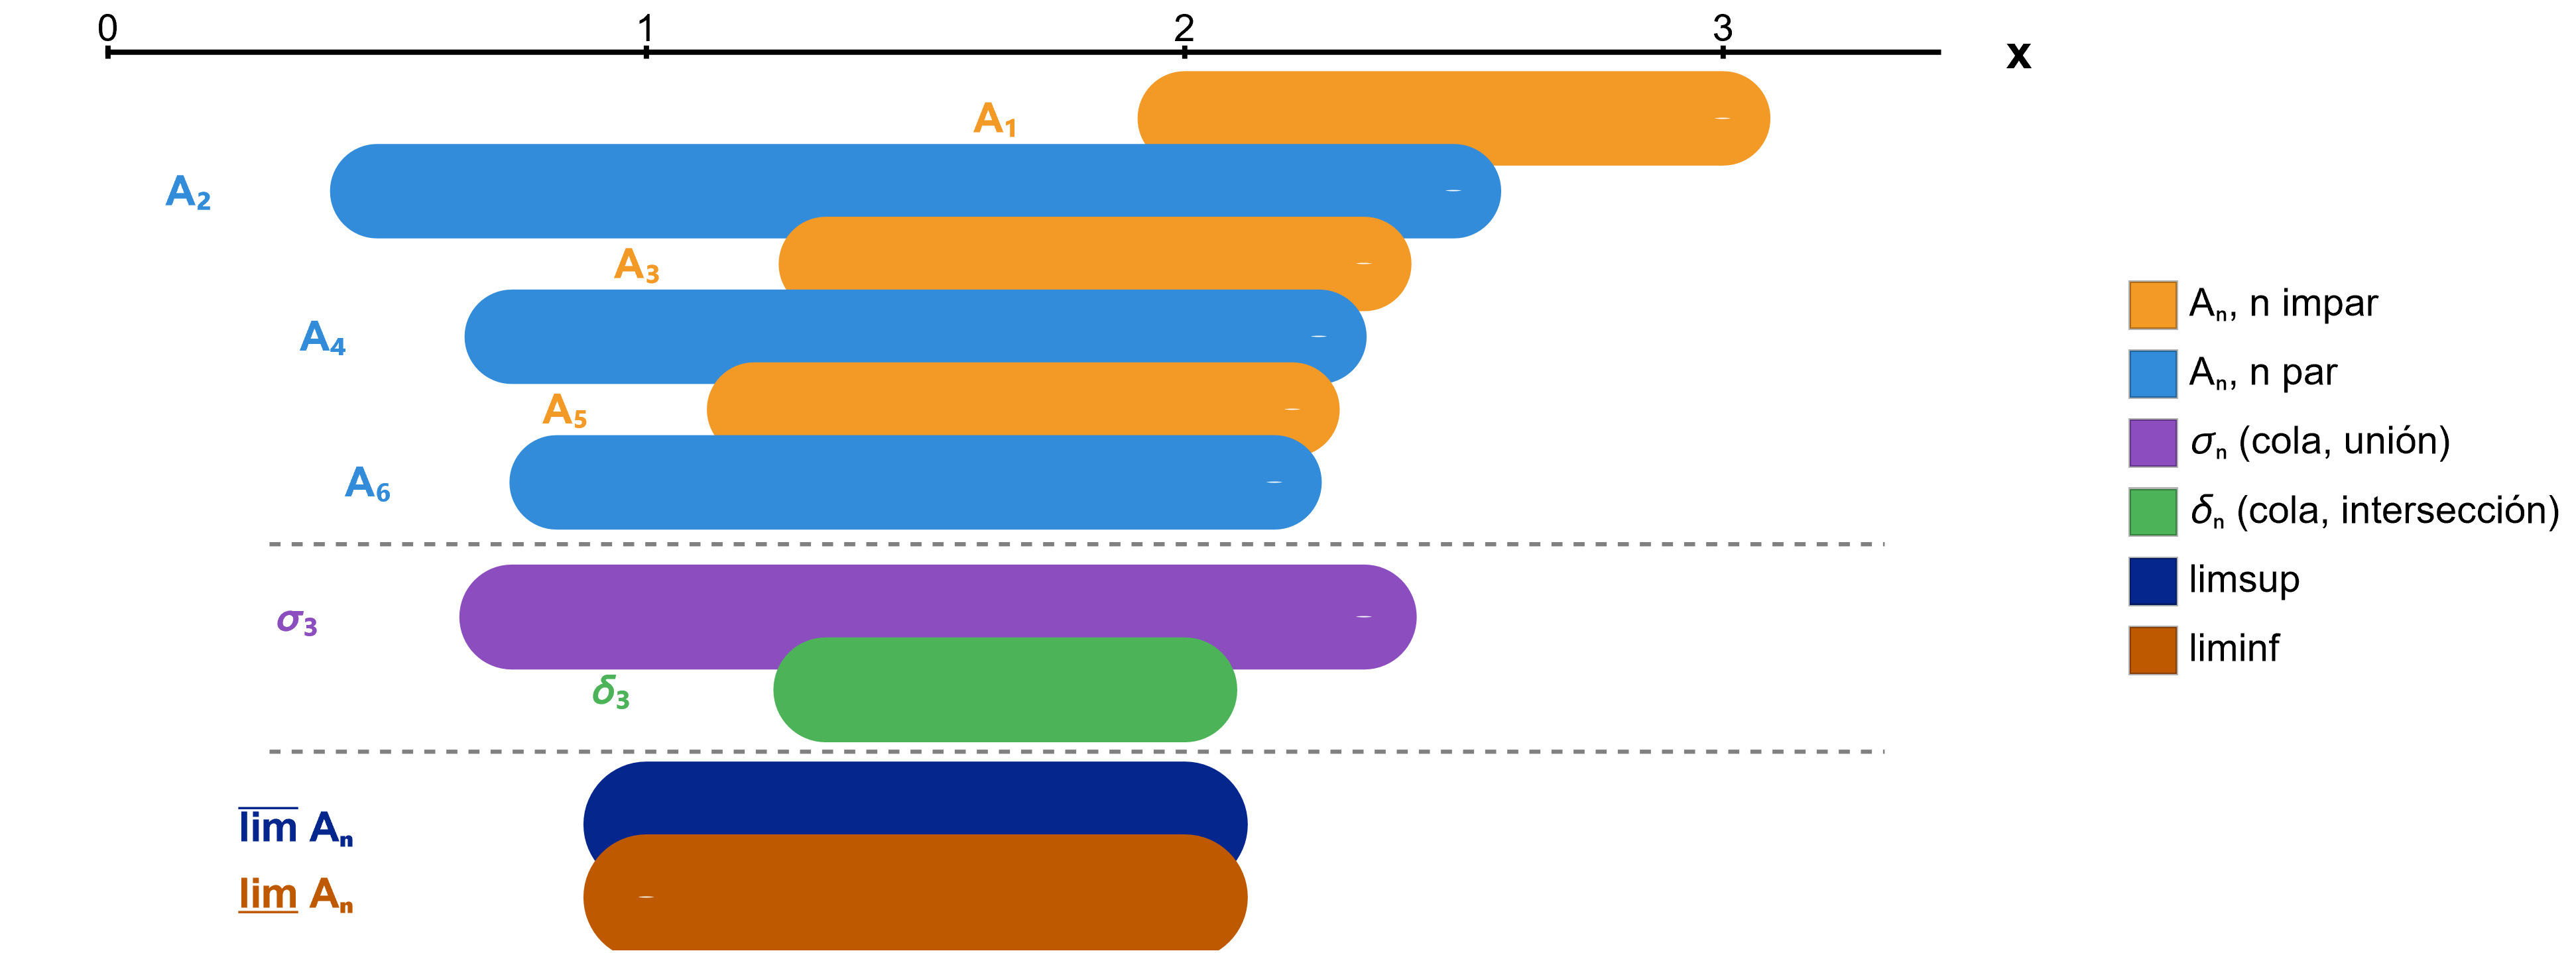
\includegraphics[width=0.85\linewidth]{imagenes/examenes_resueltos/propuesto1_P1.png}
\end{center}

\paragraph{b) Demostración de que $P_X$ es una medida sobre $(\Omega_2, \mathcal{G}_2)$:}
Verificamos las propiedades de medida para $P_X(B) = \mu(X^{-1}(B))$:
\begin{enumerate}[label=\arabic*.]
    \item \textbf{No negatividad:} Para todo $B \in \mathcal{G}_2$, $X^{-1}(B) \in \mathcal{G}_1$. Como $\mu \ge 0$:
    \[
        P_X(B) = \mu(X^{-1}(B)) \ge 0
    \]
    \item \textbf{Conjunto vacío:} Dado que $X^{-1}(\varnothing) = \varnothing$ y $\mu(\varnothing) = 0$:
    \[
        P_X(\varnothing) = \mu(X^{-1}(\varnothing)) = \mu(\varnothing) = 0
    \]
    \item \textbf{$\sigma$-aditividad:} Sea $(B_n)_{n \in \mathbb{N}} \subseteq \mathcal{G}_2$ una sucesión de conjuntos disjuntos dos a dos ($B_i \cap B_j = \varnothing$ para $i \neq j$). Sus antiimágenes son también disjuntas dos a dos en $\Omega_1$:
    \[
        X^{-1}(B_i) \cap X^{-1}(B_j) = X^{-1}(B_i \cap B_j) = X^{-1}(\varnothing) = \varnothing, \quad \forall i \neq j
    \]
    Por la $\sigma$-aditividad de la medida $\mu$:
    \[
        P_X\left( \bigcup_{n=1}^\infty B_n \right) = \mu\left( X^{-1}\left( \bigcup_{n=1}^\infty B_n \right) \right) = \mu\left( \bigcup_{n=1}^\infty X^{-1}(B_n) \right) = \sum_{n=1}^\infty \mu(X^{-1}(B_n)) = \sum_{n=1}^\infty P_X(B_n)
    \]
\end{enumerate}

\paragraph{c) Medida de probabilidad inducida:}
Si $\mu$ es una probabilidad ($\mu(\Omega_1) = 1$), evaluamos $P_X$ en el espacio total $\Omega_2$:
\[
    P_X(\Omega_2) = \mu(X^{-1}(\Omega_2)) = \mu(\Omega_1) = 1
\]
Por lo tanto, $P_X$ es una medida de probabilidad sobre $(\Omega_2, \mathcal{G}_2)$.
\end{problema}

\newpage %===

% ------------------------------------------------------------------------------
% PROBLEMA 4
% ------------------------------------------------------------------------------
\begin{problema}[Descomposición de Lebesgue de una función de distribución y esperanza]
Se considera la función $F : \mathbb{R} \to [0, 1]$ definida por:
\[
    F(x) = \begin{cases} 
        0 & \text{si } x < 0 \\
        \dfrac{1}{4} + \dfrac{x}{2} & \text{si } 0 \le x < 1 \\
        1 & \text{si } x \ge 1
    \end{cases}
\]
\begin{enumerate}[label=\alph*)]
    \item Demostrar que $F$ es una función de distribución propia sobre $\mathbb{R}$.
    \item Hallar el conjunto de puntos de discontinuidad $D$ y determinar la descomposición única $F = \alpha F_D + (1-\alpha) F_C$, identificando la constante $\alpha \in [0,1]$, la función de distribución discreta $F_D$ y la continua $F_C$.
    \item Sea $X$ una variable aleatoria con función de distribución $F_X = F$. Calcular las probabilidades $P(X = 0)$, $P(X = 1)$ y $P\left(X \in \left[0, \frac{1}{2}\right]\right)$.
    \item Calcular la esperanza matemática $E[X]$.
\end{enumerate}

\tcblower

\paragraph{a) Comprobación de las propiedades de función de distribución:}
\begin{enumerate}[label=\arabic*.]
    \item \textbf{Monotonía creciente:} En cada tramo $F$ es constante o lineal con pendiente positiva ($1/2 > 0$). En los puntos de cambio de tramo: $0 \le 1/4 \le 3/4 \le 1$. Luego $F(x) \le F(y)$ para todo $x \le y$.
    \item \textbf{Continuidad por la derecha:}
    $\lim_{x \to 0^+} F(x) = \frac{1}{4} = F(0)$ y $\lim_{x \to 1^+} F(x) = 1 = F(1)$. En el resto de puntos $F$ es continua.
    \item \textbf{Límites en el infinito:} $\lim_{x \to -\infty} F(x) = 0$ y $\lim_{x \to +\infty} F(x) = 1$.
\end{enumerate}
Por lo tanto, $F$ es una función de distribución propia.

\paragraph{b) Descomposición $F = \alpha F_D + (1-\alpha) F_C$:}
Identificamos los puntos de salto $D = \{0, 1\}$ y la magnitud de sus saltos $s_i = F(x_i) - F(x_i^-)$:
\begin{itemize}
    \item En $x = 0$: $s_1 = F(0) - F(0^-) = \frac{1}{4} - 0 = \frac{1}{4}$.
    \item En $x = 1$: $s_2 = F(1) - F(1^-) = 1 - \frac{3}{4} = \frac{1}{4}$.
\end{itemize}

La masa discreta total viene dada por $\alpha = s_1 + s_2 = \frac{1}{4} + \frac{1}{4} = \frac{1}{2}$.

Construimos la función de salto acumulada $G(x) = \sum_{x_i \le x} s_i$:
\[
    G(x) = \begin{cases} 0 & \text{si } x < 0 \\ \dfrac{1}{4} & \text{si } 0 \le x < 1 \\ \dfrac{1}{2} & \text{si } x \ge 1 \end{cases}
    \implies 
    F_D(x) = \frac{G(x)}{\alpha} = \begin{cases} 0 & \text{si } x < 0 \\ \dfrac{1}{2} & \text{si } 0 \le x < 1 \\ 1 & \text{si } x \ge 1 \end{cases}
\]

\begin{center}
    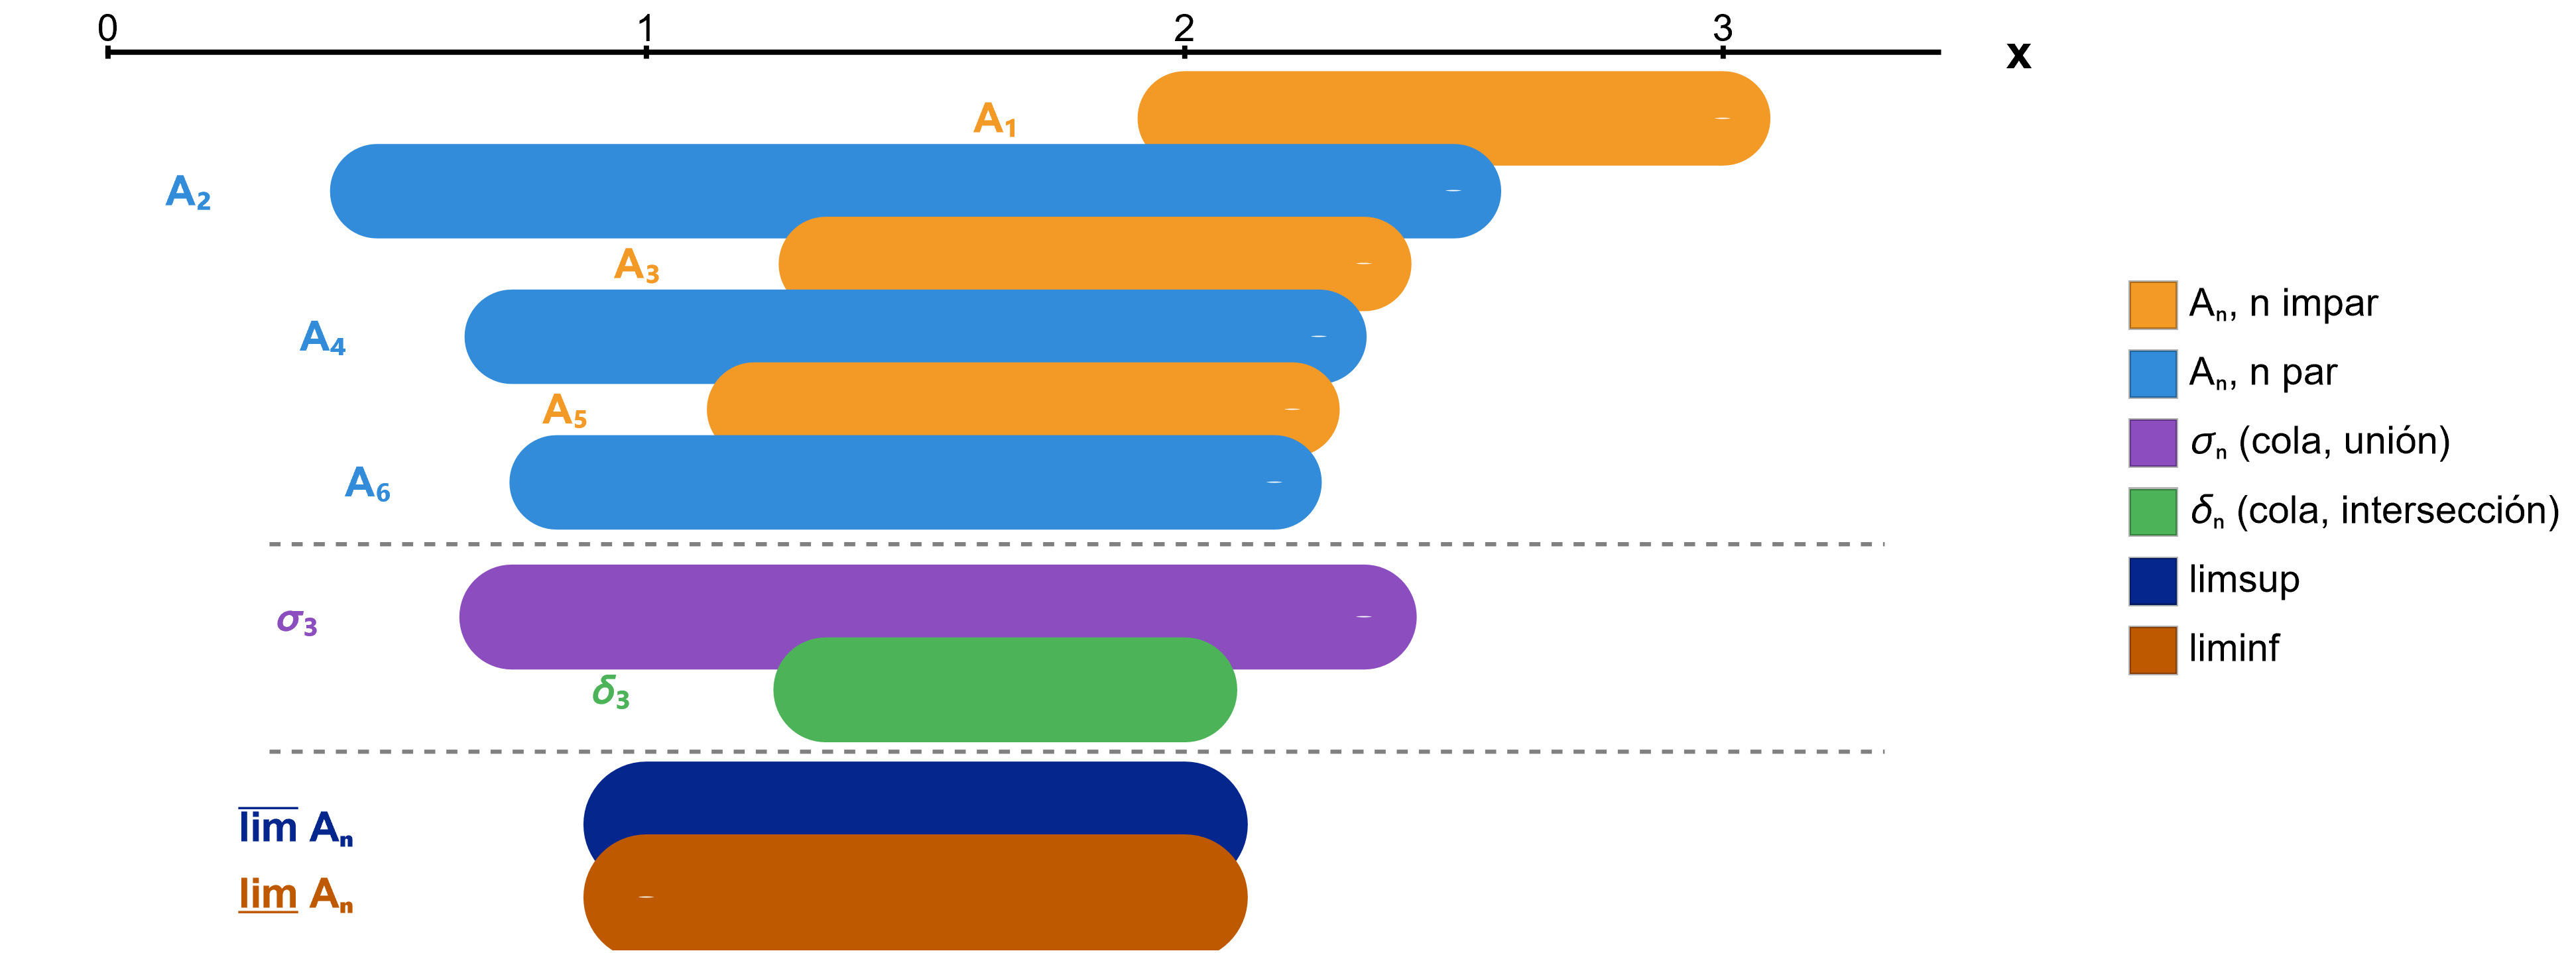
\includegraphics[width=0.85\linewidth]{imagenes/examenes_resueltos/propuesto1_P1.png}
\end{center}
Para la parte continua, calculamos $H(x) = F(x) - G(x)$:
\[
    H(x) = \begin{cases} 0 & \text{si } x < 0 \\ \dfrac{x}{2} & \text{si } 0 \le x < 1 \\ \dfrac{1}{2} & \text{si } x \ge 1 \end{cases}
    \implies 
    F_C(x) = \frac{H(x)}{1-\alpha} = \begin{cases} 0 & \text{si } x < 0 \\ x & \text{si } 0 \le x < 1 \\ 1 & \text{si } x \ge 1 \end{cases}
\]
donde $F_C(x)$ representa la función de distribución uniforme en $[0, 1]$. La descomposición es:
\[
    F(x) = \frac{1}{2} F_D(x) + \frac{1}{2} F_C(x)
\]

\paragraph{c) Cálculo de probabilidades:}
\begin{itemize}
    \item $P(X = 0) = F(0) - F(0^-) = \frac{1}{4} - 0 = \frac{1}{4}$.
    \item $P(X = 1) = F(1) - F(1^-) = 1 - \frac{3}{4} = \frac{1}{4}$.
    \item $P\left(X \in \left[0, \frac{1}{2}\right]\right) = F\left(\frac{1}{2}\right) - F(0^-) = \left( \frac{1}{4} + \frac{1}{4} \right) - 0 = \frac{1}{2}$.
\end{itemize}

\paragraph{d) Cálculo de la esperanza $E[X]$:}
Utilizando la descomposición de la esperanza $E[X] = \alpha E[X_D] + (1-\alpha) E[X_C]$:
\begin{itemize}
    \item Parte discreta: $E[X_D] = 0 \cdot P_D(X_D = 0) + 1 \cdot P_D(X_D = 1) = 0 \cdot \frac{1}{2} + 1 \cdot \frac{1}{2} = \frac{1}{2}$.
    \item Parte continua (con densidad $f_C(x) = \mathbf{1}_{[0,1]}(x)$): $E[X_C] = \int_0^1 x \cdot 1 \, dx = \left[ \frac{x^2}{2} \right]_0^1 = \frac{1}{2}$.
\end{itemize}
Sustituyendo obtenemos:
\[
    E[X] = \frac{1}{2} \left( \frac{1}{2} \right) + \frac{1}{2} \left( \frac{1}{2} \right) = \frac{1}{4} + \frac{1}{4} = \frac{1}{2}
\]
\end{problema}